\documentclass[11pt,letterpaper]{article}
\usepackage[margin=1in]{geometry}
\usepackage[T1]{fontenc}
\usepackage{lmodern,microtype}
\usepackage{amsmath,amssymb,booktabs,longtable,array}
\usepackage{graphicx,xcolor,listings,enumitem,placeins}
\usepackage[font=small,labelfont=bf]{caption}
\usepackage[colorlinks=true,linkcolor=blue!45!black,urlcolor=blue!45!black,
  citecolor=blue!45!black]{hyperref}
\usepackage{fancyhdr}
\definecolor{ink}{RGB}{28,48,66}
\definecolor{codebg}{RGB}{246,248,250}
\lstdefinestyle{stata}{basicstyle=\ttfamily\footnotesize,
  backgroundcolor=\color{codebg},frame=single,rulecolor=\color{black!15},
  breaklines=true,columns=fullflexible,keepspaces=true,
  showstringspaces=false,upquote=true,aboveskip=10pt,belowskip=10pt}
\lstset{style=stata}
\newcommand{\code}[1]{\texttt{\detokenize{#1}}}
\newcolumntype{P}[1]{>{\raggedright\arraybackslash}p{#1}}
\newcommand{\E}{\mathbb{E}}
\newcommand{\Var}{\operatorname{Var}}
\newcommand{\Cov}{\operatorname{Cov}}
\setlength{\emergencystretch}{2em}
\setlength{\parskip}{5pt}
\setlength{\parindent}{0pt}
\setlist{itemsep=2pt,topsep=4pt}
\pagestyle{fancy}
\fancyhf{}
\fancyhead[L]{\small\color{ink}\textsf{fesim: User and Technical Manual}}
\fancyhead[R]{\small\textsf{1.2.0-rc.1}}
\fancyfoot[C]{\thepage}
\setlength{\headheight}{14pt}
\hypersetup{pdftitle={fesim: User and Technical Manual},
 pdfauthor={Johannes F. Schmieder},
 pdfsubject={Linked employer-employee simulation in Stata and Mata}}
\begin{document}
\hypersetup{pageanchor=false}
\begin{titlepage}
\vspace*{0.8in}
{\color{ink}\Huge\bfseries fesim\par}
\vspace{0.3in}
{\LARGE User and Technical Manual\par}
\vspace{0.15in}
{\large Linked employer--employee panel simulation in Stata\par}
\vspace{0.5in}
Johannes F. Schmieder\\
Boston University
\vspace{0.35in}

Development version 1.2.0-rc.1 \quad $\cdot$ \quad Mata API 37\\
September 30, 2026
\vspace{0.5in}

\begin{minipage}{0.91\textwidth}
This manual explains the public command, all ten available presets, and the
data and diagnostics they return. Reproducible examples illustrate wage
dispersion, sorting, pay gaps, search dynamics, and wage bargaining. The technical appendix
documents the implemented random processes and derives the canonical
Burdett--Mortensen equilibrium, its finite-firm approximation, and the exact
continuous-time worker simulation. A further appendix derives CPV values,
contract wages, incumbent raises, and joint stationary histories. The BLM
appendix defines finite worker and firm types, nonadditive earnings,
endogenous mobility, and persistent monthly wage histories.

This manual accompanies the untagged \code{1.2.0-rc.1} candidate.
Qualification is limited to Stata/MP 19 on macOS Apple Silicon; exact source
and archive evidence are recorded in the repository qualification guide.
The stable \code{v0.1.0} release contains the earlier simple-AKM command.
\end{minipage}
\vfill
\url{https://github.com/johannes-schmieder/fesim}\\
\url{https://johannes-schmieder.com/}\\
MIT License
\end{titlepage}
\pagenumbering{roman}
\hypersetup{pageanchor=true}
\tableofcontents
\clearpage
\pagenumbering{arabic}

\section{What the command produces}
\code{fesim} creates synthetic linked employer--employee data. Each row is a
worker observed in a retained output period, including periods of
nonemployment. Worker identifiers stay fixed; employers can change; wages
are observed only when employed. The command separates the economic DGP,
its numerical preset, the destination network, and the observation frequency.
It supports teaching, Monte Carlo experiments, and evaluation of estimators
whose behavior depends on mobility and worker--firm sorting.

The installed engine uses official Stata and Mata only. Stata 19 is the
supported minimum. The current development source has been qualified on
Stata/MP 19 on macOS Apple Silicon; Windows qualification of the older
\code{v0.1.0} release does not qualify the later BM, CPV or BLM implementations.
Reproducibility claims refer to a fixed package source, seed, command, and
qualified Stata environment.

\subsection{Choose a DGP}
\begin{longtable}{@{}P{0.24\textwidth}P{0.22\textwidth}P{0.47\textwidth}@{}}
\toprule
Family / preset & Short name & Purpose and interpretation\\
\midrule
\endhead
\code{akm / simple} & \code{akmsimple} &
Additive worker and firm effects, independent attraction weights, and
discrete interval mobility. Stylized teaching and testing baseline.\\[4pt]
\code{akm / stylized} & \code{akmempirical} &
Monthly mobility with latent worker types, firm quality, duration dependence,
and sorting. All defaults are stylized; the alias names the mechanism.\\[4pt]
\code{akm /}\newline{\footnotesize\code{germany_chk_2002_2009}} & None &
The monthly engine with selected West German wage-dispersion and
sorting targets from Card, Heining, and Kline (CHK).\\[4pt]
\code{akmpaygap / simple} & None &
Two groups with different worker distributions, premium schedules,
mobility probabilities, and sorting. Stylized.\\[4pt]
\code{akmpaygap / cck2016} & None &
Targets selected Card, Cardoso, and Kline (CCK) group moments and
male-reference firm decomposition under the package normalization.\\[4pt]
\code{bm / simple} & \code{bmsimple} &
Homogeneous-worker, common-productivity wage posting with unemployed and
on-the-job search. Exact continuum model; stylized primitives.\\[4pt]
\code{cpv / simple} & None &
Sequential wage bargaining, incumbent raises, heterogeneous firms and
homogeneous workers. Stylized primitives.\\[4pt]
\code{cpv / heterogeneous} & None &
The same bargaining engine with mean-one lognormal worker ability.
No endogenous ability sorting.\\[4pt]
\code{blm / static} & None &
Finite worker types and firm classes, nonadditive Gaussian cell earnings,
and type-dependent sorting. Employed workers only.\\[4pt]
\code{blm / dynamic} & None &
The same finite economy with persistent earnings, wage-dependent moves
and origin-class move shifts. Flexible, uncalibrated primitives.\\
\bottomrule
\end{longtable}

There are five canonical family names and ten family/preset combinations.
The three aliases resolve to designated presets. Omitting \code{dgp()}
and \code{preset()} selects \code{akm/simple}.
AKM terminology follows Abowd, Kramarz, and Margolis \cite{akm}.
The search model follows Burdett and Mortensen's wage-posting framework
\cite{bm}; its specific discounted-worker reservation condition and
implementation are derived in Appendix~\ref{app:bm}.

\subsection{Install and begin}
To use all designs in this manual, install the development package from the
repository root in Stata. A checkout also permits source-based use:
\begin{lstlisting}
* Change this path to your local checkout.
cd "/path/to/fesim"
adopath ++ "."
help fesim
fesim version
fesim list
fesim presets akm
fesim describe bm, preset(simple)
\end{lstlisting}
The installed help contains numbered \emph{click to run} links. Each invokes
\code{fesim_run}, runs a whole example, and restores the caller's dataset.
The source-only loader can compile packaged Mata sources when a compatible
library is absent. The README gives development and immutable stable-tag
installation instructions.

\section{Syntax and options}\label{sec:syntax}
\begin{lstlisting}
fesim [, dgp(name) preset(name)
    workers(#) firms(#) periods(#)
    frequency(year|quarter|month) start(date) seed(#)
    initial(stationary|random|allunemployed) burnin(#)
    jobrule(end) truth(none|basic|full)
    connectivity(keep|largest) network(random|blocks|bridges|ladder)
    parameters(name value [name value ...]) report noreport clear]

fesim version
fesim list
fesim presets [dgp]
fesim describe dgp [, preset(name)]
\end{lstlisting}
The display lists alternatives: \code{report} and \code{noreport} are
mutually exclusive, and not every initial state or network is available
for every family. Use full option spellings in reproducible scripts.
\code{fesim} generates a population; it does not accept a variable list
or use the current dataset as an economic input.

\subsection{Common controls}
\begin{longtable}{@{}P{0.25\textwidth}P{0.68\textwidth}@{}}
\toprule
Option & Meaning\\
\midrule
\endhead
\code{dgp(name)}, \code{preset(name)} &
Resolve a family/alias and a preset. Names are case-insensitive.
\code{fesim describe} reports defaults, bounds, and provenance.\\[4pt]
\code{workers(n)}, \code{firms(n)} &
Generated workers and firm universe. Inactive firms need not appear.
Filtering may reduce returned workers without changing requested parameters.\\[4pt]
\code{periods(n)} &
Retained snapshots per worker. Monthly \code{periods(60)} covers five years.
Workers times periods cannot exceed 2,147,483,647; memory or edition limits
may bind sooner.\\[4pt]
\code{frequency(...)} &
Output interval: year (default), quarter, or month.
Changing frequency does not reinterpret annual input rates.\\[4pt]
\code{start(date)} &
First retained snapshot label: \code{2000}, \code{2000q1}, or
\code{2000m1}, for example. Default is the first period of 2000,
except Germany and CCK presets, which use 2002.\\[4pt]
\code{seed(n)} &
Integer from 0 to 2,147,483,647. Explicit seeds preserve caller RNG
state. If omitted, one caller RNG draw supplies the master seed.\\[4pt]
\code{initial(...)}, \code{burnin(n)} &
Initial state and discarded pre-sample time. Availability and units
are model-specific; see Table~\ref{tab:defaults}.\\[4pt]
\code{jobrule(end)} &
Employer at the output endpoint. Dominant- and longest-employer rules
are not public interfaces.\\[4pt]
\code{truth(...)} &
\code{none} suppresses latent columns; \code{basic} (default) adds wage
components; \code{full} adds model-specific quantities.
Economic draws are invariant to this choice.\\[4pt]
\code{connectivity(...)} &
\code{keep} (default) returns all workers. \code{largest} retains complete
histories in the selected observed component. \code{force} is unavailable.\\[4pt]
\code{network(...)} &
Destination rule. \code{random} is the default and the only allowed
design for pay-gap, BM, CPV and BLM. All four designs are available for AKM.\\[4pt]
\code{parameters(...)} &
Whitespace-separated name/value pairs; BLM also accepts Stata matrix names. Model and network controls
belong here. Unknown, duplicate, irrelevant, conflicting, or inadmissible
inputs fail validation. Numeric common controls also accept this input route;
named options are preferred and duplicate specification is rejected.\\[4pt]
\code{report}, \code{noreport} &
Show (default) or suppress the report without changing data.\\[4pt]
\code{clear} &
Authorize replacement of loaded data. Without it, the command rejects
a run that would replace the caller's dataset.\\
\bottomrule
\end{longtable}

\setcounter{table}{0}
\begin{table}[htbp]
\centering\small
\caption{Population, timing, and initialization defaults}\label{tab:defaults}
\begin{tabular}{@{}lrrrll@{}}
\toprule
Preset & Workers & Firms & Periods & Initial & Burn-in\\
\midrule
AKM simple & 10,000 & 500 & 10 & stationary & 0 intervals\\
AKM stylized & 10,000 & 500 & 10 & random & 5 years\\
AKM Germany & 10,000 & 1,000 & 8 & random & 5 years\\
Pay-gap simple & 10,000 & 500 & 10 & random & 5 years\\
Pay-gap CCK & 10,000 & 1,000 & 8 & random & 5 years\\
BM simple & 10,000 & 500 & 10 & stationary & 0 years\\
CPV (both) & 10,000 & 500 & 10 & stationary & 0 years\\
BLM (both) & 10,000 & 500 & 10 & random & 20 years\\
\bottomrule
\end{tabular}
\end{table}
All presets except BLM support \code{initial(allunemployed)}. Exact stationary starts
are available for simple AKM, BM and both CPV presets. Random starts require at least one
burn-in output interval for simple AKM and at least one year for monthly
AKM and pay-gap. Those AKM/pay-gap burn-in inputs are integers. BM and CPV burn-in is
continuous years and can be fractional. Pay-gap uses output-clock steps
within its year-valued burn-in. BLM permits only random starts; its burn-in
is year-valued, nonnegative and aligned to whole months, with a 20-year default.
Finite burn-in does not certify stationarity.

\paragraph{Discovery and compatibility.}
\code{fesim describe} also reports observed and truth-variable inventories,
applicable initialization and network choices, parameter units, and scientific
source/target scope. Full-truth inventories list additions beyond basic truth;
conditional network fields are separate. Existing v1 option meanings, defaults,
output semantics, and named matrices are compatibility commitments. Numerical
fixes that change seeded output must be disclosed. See
\href{https://github.com/johannes-schmieder/fesim/blob/main/docs/compatibility.md}{the compatibility policy}
for accepted option abbreviations and future deprecation rules.

\subsection{Changing model parameters}
\begin{lstlisting}
preserve
fesim, dgp(akm) preset(simple) workers(1000) firms(50) ///
    periods(8) seed(12345) ///
    parameters(sd_worker .45 sd_firm .20 p_ee .25) clear
matrix list r(parameters)
restore
\end{lstlisting}
The matrix has \code{value}, \code{default}, \code{lower}, and \code{upper}
columns; cross-parameter restrictions also apply. Common scalar dimensions
use named options. Model overrides change \code{stylized} to
\code{stylized_modified}, or \code{targeted} to \code{targeted_modified}.
Inspect \code{r(calibration_class)} and dataset characteristics when
documenting an experiment.

\section{DGP parameter reference}\label{sec:parameters}
\subsection{Simple AKM}
Employed log wages satisfy
\begin{equation}
y_{it}=\mu+\alpha_i+\psi_{J_{it}}+\gamma\,t_{\rm years}+\epsilon_{it}.
\label{eq:akm}
\end{equation}
Worker effects, firm effects, attraction, and wage errors use separate
primitives. Default random destinations do not condition on ability or pay.
\begin{center}\small
\begin{tabular}{@{}llr@{}}
\toprule
Parameter & Meaning & Default\\
\midrule
\code{mu} & Mean log-wage intercept & 3\\
\code{sd_worker} & Worker-effect SD & .40\\
\code{sd_firm} & Firm-effect SD & .15\\
\code{sd_error} & Idiosyncratic log-wage SD & .20\\
\code{firm_size_sd} & Log attraction scale & 1\\
\code{p_eu}, \code{p_ee}, \code{p_ue} & Annual probabilities & .08, .12, .60\\
\code{wage_trend} & Log points per retained-sample year & 0\\
\bottomrule
\end{tabular}\end{center}
SDs are nonnegative. EU and EE probabilities are nonnegative and sum to
less than one; UE lies in $[0,1]$. Positive EE requires at least two firms.
Stationary initialization is undefined when both EU and UE are zero.

\subsection{Monthly AKM: stylized and Germany}
The stylized preset retains the wage and attraction defaults above but
replaces interval probabilities by monthly transitions from annual hazards.
\begin{longtable}{@{}P{0.44\textwidth}P{0.21\textwidth}P{0.28\textwidth}@{}}
\toprule
Parameter & Stylized default & Role\\
\midrule
\endhead
\code{rho_z_alpha}, \code{rho_q_psi} & .30, .50 & Latent correlations\\
\code{kappa_eu} & $-2.416230719$ & EU log-hazard intercept\\
\code{eu_worker}, \code{eu_firm}, \code{eu_duration} & .10, $-.10$, $-.20$ &
EU type, quality, duration slopes\\
\code{kappa_ee} & $-2.010765611$ & EE log-hazard intercept\\
\code{ee_worker}, \code{ee_firm}, \code{ee_duration} & .10, $-.10$, $-.15$ &
EE type, quality, duration slopes\\
\code{kappa_ue} & $-.087421572$ & UE log-hazard intercept\\
\code{ue_worker}, \code{ue_duration} & .15, $-.25$ & UE slopes\\
\code{theta_sort}, \code{theta_quality} & .25, .10 & Sorting / quality preference\\
\code{theta_up}, \code{theta_down} & .20, $-.10$ & Asymmetric EE distances\\
\bottomrule
\end{longtable}
Exact intercepts are the logs of $-\log(1-.08-.12)$ split in .08/.12
proportions and of $-\log(1-.60)$ for UE. Monthly presets do not accept
\code{p_eu}, \code{p_ee}, or \code{p_ue}. Correlations lie in $[-1,1]$;
a zero wage-effect SD requires its corresponding latent correlation to be
zero. Other numerical bounds are available through \code{fesim describe}.

The Germany preset changes \code{sd_worker} to .357, \code{sd_firm} to
.230, \code{sd_error} to .135, and \code{theta_sort} to 2.2. The first
three values are CHK component targets; sorting targets employed-observation
covariance .0205, half the reported $2\Cov=.041$ \cite{chk}.
Hazards and durations remain stylized. This is a targeted wage-dispersion
and sorting design, not a reconstruction of German employment histories.

\subsection{Pay-gap presets}
Men are \code{group=0}, women \code{group=1}; gaps are men minus women.
Each firm has surplus $s_j\sim N(0,1)$ and group premium
\[
\psi_{gj}=a_g+b_gs_j+\tau_g\eta_{gj},\qquad
y_{it}=\mu_g+\alpha_i+\psi_{gJ_{it}}+\gamma_g t_{\rm years}+\epsilon_{it}.
\]
Surplus is not restandardized in the finite sample. Both schedules exist at
each firm, even when only one group is observed there.
\begin{longtable}{@{}P{0.47\textwidth}rr@{}}
\toprule
Parameter (men, women where paired) & Simple & CCK\\
\midrule
\endhead
\code{female_share} & .50 & .46\\
\code{mu_m}, \code{mu_f} & 3, 2.9 & 3, 2.815\\
\code{sd_worker_m}, \code{sd_worker_f} & .40, .40 & .420, .400\\
\code{premium_intercept_m}, \code{premium_intercept_f} & .05, .03 & .113, .099\\
\code{premium_loading_m}, \code{premium_loading_f} & .15, .12 & .247, .12567\\
\code{premium_deviation_sd_m}, \code{premium_deviation_sd_f} &
0, .09 & 0, .1719768912\\
\code{sd_error_m}, \code{sd_error_f} & .20, .20 & .143, .125\\
\code{firm_size_sd} & 1 & 1\\
\code{p_eu_m}, \code{p_eu_f} & .08, .08 & .08, .08\\
\code{p_ee_m}, \code{p_ee_f} & .12, .12 & .12, .12\\
\code{p_ue_m}, \code{p_ue_f} & .60, .60 & .60, .60\\
\code{group_sort_m}, \code{group_sort_f} & .30, 0 & .142, 0\\
\code{worker_sort_m}, \code{worker_sort_f} & .30, .30 & .18, .273\\
\code{wage_trend_m}, \code{wage_trend_f} & 0, 0 & .05, .05\\
\bottomrule
\end{longtable}
Groupwise competing-probability restrictions are the same as in simple AKM;
at least two firms are required. \code{female_share} lies in $[0,1]$.
Group moments are undefined when the relevant group/sample is empty.
The CCK preset targets selected group wage/effect moments and a male-reference
decomposition \cite{cck}. Its standard-normal-surplus normalization differs
from CCK's low-surplus-firm normalization. Targets are not constraints forcing
each realized sample to reproduce published moments.

\subsection{Burdett--Mortensen}
\begin{center}\small
\begin{tabular}{@{}llrl@{}}
\toprule
Parameter & Economic meaning & Default & Unit\\
\midrule
\code{b} & Unemployment flow payoff & .4 & Wage level\\
\code{p} & Common productivity & 1 & Wage level\\
\code{lambda_u} & Unemployed offer rate & 1 & Annual rate\\
\code{lambda_e} & Employed offer rate & .5 & Annual rate\\
\code{delta} & Job destruction rate & .2 & Annual rate\\
\code{r} & Worker discount rate & .05 & Annual rate\\
\code{random_firms} & 0 midpoint / 1 random quantiles & 0 & Indicator\\
\bottomrule
\end{tabular}\end{center}
Rates must be positive and at most 1,000. Productivity must exceed $b$,
and solved wage support must be positive because output wages are logs.
Support and residual checks can reject numerically unresolved inputs.
There is no public control for measurement error, heterogeneous productivity,
bargaining, or firm attraction.

The continuum equilibrium is solved first. Finite posted wages discretize
its offer distribution. Workers contact finite firms uniformly and accept
only strictly higher wages while employed. The exact finite stationary
allocation differs from the continuum worker distribution; a finite
wage-posting game is not solved anew (Appendix~\ref{app:bm}).

\subsection{Cahuc--Postel-Vinay--Robin bargaining}\label{sec:cpvparams}
\code{dgp(cpv)} implements the sequential bargaining protocol of
Cahuc, Postel-Vinay, and Robin \cite{cpv} in a finite firm economy.
\code{preset(simple)} has identical workers; \code{preset(heterogeneous)}
adds mean-one lognormal worker ability. Both have heterogeneous firms.
These are stylized designs, not estimates or a replication of the paper.
\begin{center}\small
\begin{tabular}{@{}llrl@{}}
\toprule
Parameter & Meaning & Default & Unit\\
\midrule
\code{b} & Unemployment flow payoff & 1 & Per efficiency unit\\
\code{p_min}, \code{p_max} & Uniform firm productivity support & 1.5, 2 & Per efficiency unit\\
\code{lambda_u} & Unemployed offer rate & .5 & Per year\\
\code{lambda_e} & Employed offer rate & .3 & Per year\\
\code{delta} & Destruction rate & .2 & Per year\\
\code{r} & Discount rate & .05 & Per year\\
\code{beta} & Worker bargaining share & .5 & Share in $[0,1]$\\
\code{sd_worker} & Log ability standard deviation & 0 or .4 & Log units\\
\code{random_firms} & Midpoint (0) or random (1) quantiles & 0 & Indicator\\
\bottomrule
\end{tabular}\end{center}
The heterogeneous preset changes only \code{sd_worker} to .4. All model
controls belong in \code{parameters()}, for example:
\begin{lstlisting}
fesim, dgp(cpv) preset(heterogeneous) workers(5000) firms(100) ///
    periods(60) frequency(month) seed(12345) truth(full) ///
    parameters(beta .3 sd_worker .5 lambda_e .4) clear
\end{lstlisting}
Firm productivity must be positive with $p_{\max}\ge p_{\min}$; equal
endpoints are allowed. The unemployed offer, destruction, and discount
rates are positive and at most 1,000; the employed offer rate may be zero.
The flow payoff is positive and ability dispersion is nonnegative.
Every generated firm must have strictly positive full surplus and entry
wage. The solver rejects an invalid economy without clipping wages or
removing firms. Random firm draws are included in transactional rollback.

Defaults are 10,000 workers, 500 firms, ten annual observations,
\code{initial(stationary)} and zero burn-in for both presets.
Stationary initialization draws the joint employer, contract and tenure
state. \code{initial(random)} starts half the workers employed at random
firms with entry contracts and requires positive continuous-year burn-in.
\code{initial(allunemployed)} starts all workers with zero unemployment
age. Only \code{network(random)} and \code{jobrule(end)} are supported;
\code{connectivity(keep)} and \code{connectivity(largest)} are available.

Outside offers can raise the wage without changing the employer or spell.
A move to a more productive firm can reduce today's wage because future
bargaining opportunities improve. Worker ability multiplies production,
wages, unemployment income and values; common contact rates imply no
ability sorting. Neither structural firm productivity nor a contract wage
is an AKM firm effect. Appendix~\ref{app:cpv} derives the implementation.


\subsection{Bonhomme--Lamadon--Manresa-style finite types}\label{sec:blmparams}
\code{dgp(blm)} selects \code{preset(static)} by default. Both presets generate
employed-only panels on an internal monthly clock. Their flexible Gaussian
specification follows the static and first-order dynamic restrictions of
Bonhomme, Lamadon and Manresa \cite{blm}; it is not an implementation of their
estimator or a replication of their Swedish estimates. Appendix~\ref{app:blm}
defines the exact forward process and its relationship to the author code.

Let $l$ denote permanent worker type and $k$ firm class. Distinct actual firms
within a class share earnings and mobility primitives. Class identity is not
firm identity: moves within a class still create a new employment spell.
\begin{longtable}{@{}P{.27\textwidth}P{.20\textwidth}P{.46\textwidth}@{}}
\toprule
Scalar key & Static / dynamic & Meaning\\\midrule\endhead
\code{worker_types}, \code{firm_types} & 6, 10 (both) &
Integers $L,K$ from 1 to 20; number of actual firms $J\geq K$.\\[3pt]
\code{mu} & 3 / 3 & Grand location of log earnings.\\[3pt]
\code{sd_worker}, \code{sd_firm} & .4, .15 (both) &
Nonnegative coefficients of normalized type and class scores.\\[3pt]
\code{interaction} & .1 / .1 & Coefficient of the product of scores.\\[3pt]
\code{sd_error} & .2 / .2 & Nonnegative cell scale; fixed-cell stationary SD when persistence is nonzero.\\[3pt]
\code{lambda_move} & .25 / .25 & Nonnegative annual baseline move intensity.\\[3pt]
\code{sorting} & .5 / .5 & Type--class coefficient in destination log weights.\\[3pt]
\code{rho} & 0 / .6 & Annual persistence in $[0,1)$; monthly value $\rho^{1/12}$.\\[3pt]
\code{mobility_wage} & 0 / $-2$ & Log-intensity slope on current earnings minus origin cell location.\\[3pt]
\code{origin_dependence} & 0 / .05 & Move-shift coefficient on origin score minus destination score.\\
\bottomrule
\end{longtable}
All real inputs must be finite; coefficients without a stated sign restriction
may be negative. Static mode requires all persistence, wage-mobility and
move-shift entries to equal zero. Dynamic mode with those three components zero
reproduces static paths exactly for the same seed and remaining inputs.

Full matrices replace scalar recipes. Values are copied from ordinary Stata
matrices and validated before data or RNG mutation. Dimensions must match the
specified $L,K$; supplying a matrix does not infer dimensions. Rows and columns
are positional, regardless of Stata matrix labels.
\begin{longtable}{@{}P{.35\textwidth}P{.12\textwidth}P{.46\textwidth}@{}}
\toprule
Matrix key & Shape & Values and scalar conflicts\\\midrule\endhead
\code{worker_weights} & $1\times L$ & Strictly positive worker-type weights, normalized to probabilities.\\[3pt]
\code{firm_weights} & $1\times K$ & Strictly positive class weights used to allocate actual firms.\\[3pt]
\code{mean_matrix} & $L\times K$ & Arbitrary finite locations; conflicts with explicit \code{mu}, \code{sd_worker}, \code{sd_firm}, \code{interaction}.\\[3pt]
\code{sd_matrix} & $L\times K$ & Nonnegative scales; conflicts with \code{sd_error}.\\[3pt]
\code{move_rate_matrix} & $L\times K$ & Nonnegative annual rates; conflicts with \code{lambda_move}.\\[3pt]
\code{rho_matrix} & $L\times K$ & Annual persistence in $[0,1)$; conflicts with \code{rho}.\\[3pt]
\code{mobility_wage_matrix} & $L\times K$ & Finite log-rate slopes; conflicts with \code{mobility_wage}.\\[3pt]
\code{destination_matrix} & $(LK)\times K$ & Nonnegative class masses with positive row sums; conflicts with \code{sorting}.\\[3pt]
\code{move_shift_matrix} & $(LK)\times K$ & Finite move shifts; conflicts with \code{origin_dependence}.\\
\bottomrule
\end{longtable}
For the last two tables, row $(l-1)K+k$ identifies worker type $l$ and origin
class $k$; column $h$ is the destination class. Destination masses include the
origin employer before self-exclusion, and do not need to sum to one. An
origin-class mass is reduced by $(n_k-1)/n_k$ before renormalization. A positive
move-rate cell must have an eligible employer when $J>1$. With one actual firm,
all moves are suppressed. The initializer independently draws worker type,
a uniform actual firm, and a cell-normal wage; tenure starts at zero.

This example uses the full matrix interface with no external data:
\begin{lstlisting}
preserve
tempname M S D
matrix `M'=(2.4,2.7,3.0\3.0,3.2,3.7)
matrix `S'=(.10,.15,.20\.20,.15,.10)
matrix `D'=(1,2,3\1,2,3\1,2,3\3,2,1\3,2,1\3,2,1)
fesim, dgp(blm) workers(1000) firms(30) periods(6) ///
    seed(20260925) truth(full) parameters(worker_types 2 firm_types 3 ///
    mean_matrix `M' sd_matrix `S' destination_matrix `D') clear
matrix list r(blm_mean)
matrix list r(blm_eligible_destination)
restore
\end{lstlisting}
\code{r(parameters)} stays a numeric 16-by-4 scalar table. When a matrix replaces
a recipe, its unused scalar values are not the operative cell values. Read the
resolved \code{r(blm_*)} matrices and \code{r(blm_model)} for those values.

\section{Network designs and connectedness}\label{sec:network}
\code{network(random)} means the selected DGP's baseline destination
mechanism; empirical-AKM and pay-gap sorting can still be nonzero.
In BM and CPV it means uniform contacts with structural acceptance.
\begin{description}
\item[\code{blocks}.] Independently assign workers and firms to balanced
communities. Entry/initialization refer to the worker's home block;
EE moves refer to the current firm's block. Same-block destination mass is
multiplied by $\exp(\code{block_log_bonus})$. Defaults:
\code{block_count=4} and \code{block_log_bonus=ln(9)}. Zero bonus exactly
nests random destinations.
\item[\code{bridges}.] Ordinary moves stay strictly within blocks.
Redirect an exact number of eligible retained EE destinations across adjacent
blocks: $1\to2,2\to3,\ldots,B-1\to B$, then repeat. Distinct workers are
used. \code{bridge_count} defaults to $B-1$. Insufficient eligible events
cause failure; at least two firms per block are required.
\code{block_log_bonus} is inapplicable.
\item[\code{ladder}.] Rank firms by persistent wage effects using tied
percentile midranks. Candidates within \code{ladder_band=.10} of the origin
are lateral; lower/higher candidates outside the band are downward/upward.
Defaults \code{ladder_down_share=.10}, \code{ladder_lateral_share=.20},
and \code{ladder_up_share=.70} are renormalized over feasible directions.
Shares sum to one; ordinary destination weights apply within direction.
\end{description}
These stress designs apply only to AKM. The ladder is a reduced-form
experiment, not a structural search equilibrium. Network scalars belong
inside \code{parameters()}.

The observed bipartite graph has ever-employed workers and active firms
as nodes, and one edge per unique observed match. \code{connectivity(largest)}
selects by employed observations, then workers, firms, and smallest component
ID. Complete selected worker histories, including unemployment, are retained.
Never-employed workers are excluded; IDs are not renumbered.

\code{r(network)} has 21 rows and \code{generated}/\code{returned}
columns. It includes an undirected firm-mobility graph based on adjacent
observed direct moves. Firm links, edge-weight percentiles, articulation
firms, and graph bridges are descriptive diagnostics.

\code{r(leaveout)} separately audits the largest observed bipartite component.
Worker deletion removes complete histories. The audit repeatedly removes
articulation workers and selects the largest survivor until a robust set or
emptiness. This extends the worker-set logic in leave-out estimation
\cite{kss}. A match is vulnerable only if deletion separates firms; isolating
a stayer alone does not count. This audit does not further filter public data.

\section{Reading the panel and results}\label{sec:output}
\subsection{Observed variables}
\begin{longtable}{@{}P{0.27\textwidth}P{0.66\textwidth}@{}}
\toprule
Variable & Interpretation\\
\midrule
\endhead
\code{workerid}, \code{time} & Unique worker-period key, sorted and
balanced within returned workers. Time is Stata annual, quarterly, or monthly.\\
\code{firmid}, \code{employed} & Current firm and 0/1 employment.
Firm ID is missing in nonemployment.\\
\code{lnwage} & Log wage, missing when unemployed.
BM posted wages and CPV contract wages are levels before the logarithm.\\
\code{spellid}, \code{tenure} & Employment spell and elapsed tenure
in output-period units; missing when unemployed.\\
\code{newjob} & Changed spell from preceding snapshot; first-row missing.
Same-firm re-entry can start a new spell.\\
\code{from_unemp} & Employment after preceding-snapshot nonemployment;
first-row missing.\\
\code{to_unemp} & Employment followed by next-snapshot nonemployment;
last-row missing. This indicator is forward-looking.\\
\code{jobtojob} & Employment at different firms in adjacent snapshots;
first-row missing. It need not identify one latent EE event.\\
\code{ntransitions} & Latent state transitions in the interval;
first-row missing under the common reporting convention.\\
\code{unemp_duration} & Added by monthly AKM, BM and CPV: elapsed
unemployment duration in output units; missing when employed.\\
\code{group} & Pay-gap group: 0 Men, 1 Women.\\
\code{nbridges_imposed} & Imposed bridge events in an interval;
present for bridges under every truth mode.\\
\bottomrule
\end{longtable}
Divide durations by 1, 4, or 12 to convert output units to years.
\code{r(durations)} already uses years. BM full truth retains exact
first-interval counts even though common backward flags are first-row missing.

\subsection{Truth variables}
AKM and pay-gap basic truth includes \code{alpha_true}, \code{psi_true},
\code{time_true}, \code{xb_true}, \code{match_true}, \code{epsilon_true},
and \code{lnwage_true}. Covariate and match components are zero in current
models. Pay-gap \code{psi_true} is the observed group's premium.

Full monthly-AKM truth adds \code{worker_type_true} and
\code{firm_quality_true}; blocks/bridges add \code{worker_block_true}
and \code{firm_block_true}. Full pay-gap adds \code{firm_surplus_true},
\code{psi_male_true}, and \code{psi_female_true}.
Job-specific truth is missing when unemployed.

BM basic truth is \code{lnwage_true}, \code{posted_wage_true}, and
\code{productivity_true}; it does not fabricate AKM worker effects.
Appendix~\ref{app:bmtruth} lists full structural truth.

CPV basic truth reports log and level contract wages, worker ability, firm
productivity per efficiency unit, and match productivity. Full truth adds
bargaining references and worker values, exact offers/raises/transitions,
and employment/unemployment exposure. Worker ability remains defined during
unemployment; job attributes are missing. Appendix~\ref{app:cpv} specifies
these objects. There is no CPV structural \code{psi_true}.


\begingroup\raggedright
BLM basic truth contains \code{worker_type_true}, \code{firm_type_true},
\code{wage_location_true}, \code{conditional_mean_true}, \code{epsilon_true}
and \code{lnwage_true}. The last equals realized \code{lnwage}: there is no
additional observation error. \code{epsilon_true} is the scaled fresh
innovation, not the complete deviation from a cell location. Full truth adds
\code{lag_lnwage_true}, \code{lag_firm_type_true}, \code{persistence_true},
\code{move_shift_true}, \code{innovation_sd_true}, \code{move_probability_true},
\code{moved_month_true} and \code{n_ee_true}. Lags and conditional quantities
refer to the last internal month, even in annual data. The accounting identity is
\[
y=\mu_{lh}+\text{persistence}+\text{move shift}
+\text{innovation}.
\]
BLM returns all 13 common variables, with \code{employed=1} and
\code{unemp_duration} always missing. \code{n_ee_true} counts every actual-firm
move in the output interval, including the first interval and moves that return
to the original employer. The common first/last-row flow conventions still apply.

\par\endgroup
\subsection{Returned results}
\begingroup\small
\begin{longtable}{@{}P{0.31\textwidth}P{0.62\textwidth}@{}}
\toprule
Result & Use\\
\midrule
\endhead
\code{r(N)}, \code{r(N_workers)}, \code{r(N_firms)}, \code{r(N_firms_active)} &
Returned rows/workers, requested firms, and active firms.\\
\code{r(employment_rate)}, \code{r(p_eu_realized)}, \code{r(p_ue_realized)},
\code{r(p_ee_realized)} & Observed employment and endpoint probabilities
using appropriate origin-state denominators.\\
\code{r(parameters)} & Resolved scalar values, defaults, bounds.\\
\code{r(moments)}, \code{r(targets)} & Realized moments, applicable targets,
realized-minus-target differences, and relative differences.\\
\code{r(network)}, \code{r(leaveout)} & Graph and leave-out diagnostics.\\
\code{r(durations)} & Year-valued distributions for monthly AKM, BM and CPV:
count, mean, sample SD, p10, p50, p90.\\
\code{r(bridges)} & Eight-column imposed-event ledger.\\
\code{r(group_moments)}, \code{r(group_targets)} & Pay-gap 17-by-2 matrices.\\
\code{r(decomposition)}, \code{r(decomposition_targets)} &
Nine-by-three male, female, symmetric reference decompositions.\\
\code{r(solver)}, \code{r(bm_flows)}, \code{r(bm_firms)} &
BM solution/residuals, theory/event/endpoint flows, firm summaries.\\
\code{r(cpv_flows)}, \code{r(cpv_firms)} &
CPV finite theory, event and endpoint flows, and firm summaries;
\code{r(solver)} reports CPV Bellman values and residuals.\\
\code{r(runtime_total)}, \code{r(runtime_solve)},
\code{r(runtime_simulate)}, \code{r(runtime_output)} &
Total and stage timings in seconds.\\
\code{r(dgp)}, \code{r(preset)}, \code{r(dgp_alias)}, \code{r(seed)},
\code{r(version)}, \code{r(command)} & Identity, alias, actual master seed,
version, serialized scientific configuration.\\
\bottomrule
\end{longtable}
\endgroup
\code{r()} is transient. Copy a matrix before running another r-class
command. For example, execute \code{matrix saved_moments = r(moments)}
before \code{summarize lnwage}.

\clearpage

\begingroup\raggedright
For BLM, the 14 resolved matrices are \code{r(blm_worker_weights)},
\code{r(blm_firm_weights)}, \code{r(blm_mean)}, \code{r(blm_sd)},
\code{r(blm_move_rate)}, \code{r(blm_rho)}, \code{r(blm_mobility_wage)},
\code{r(blm_destination)}, \code{r(blm_move_shift)}, \code{r(blm_firm_counts)},
\code{r(blm_worker_scores)}, \code{r(blm_firm_scores)},
\code{r(blm_monthly_rho)} and \code{r(blm_eligible_destination)}.
\code{r(blm_cells_generated)} and \code{r(blm_cells)} have $LK$ rows and columns
\code{observations}, \code{lnwage_mean}, \code{lnwage_sd},
\code{innovation_mean}, \code{innovation_sd}, \code{interval_moves}.
They describe generated and returned samples, respectively. Moves are attributed
to the interval's ending cell. Empty means and SDs, and single-observation SDs,
are missing. \code{r(blm_workers)} gives primitive probability, generated count
and returned count by worker type. Filtering recomputes realized summaries for
complete retained worker histories; it does not redefine the primitive economy.

Full resolved values are serialized in \code{r(blm_model)} and numbered dataset
characteristics \code{_dta[fesim_blm_model_1]}, etc.; their count is
\code{_dta[fesim_blm_model_chunks]}. Matrix names are not provenance.
The short \code{r(blm_fingerprint)} is a convenience checksum with possible
collisions; use the complete serialization as the authoritative model record.
Performance scalars include \code{r(blm_worker_months)},
\code{r(blm_moves_generated)}, \code{r(blm_peak_block_rows)} and
\code{r(blm_block_workers)}, alongside the common timing scalars.

\par\endgroup
\section{Reproducible examples and figures}\label{sec:examples}
Each numbered figure example is read directly from its runnable
\code{docs/manual_examples/} do-file, so printed and executed code share
one source. Examples require \code{fesim} on the adopath and create their
own data. \code{preserve}/\code{restore} protects caller data; graphs remain
available. These illustrative samples are not calibration or estimator tests.

\subsection{Simple AKM: wages and realized sorting}
\lstinputlisting{manual_examples/01_akm.do}
\begin{figure}[!htbp]\centering
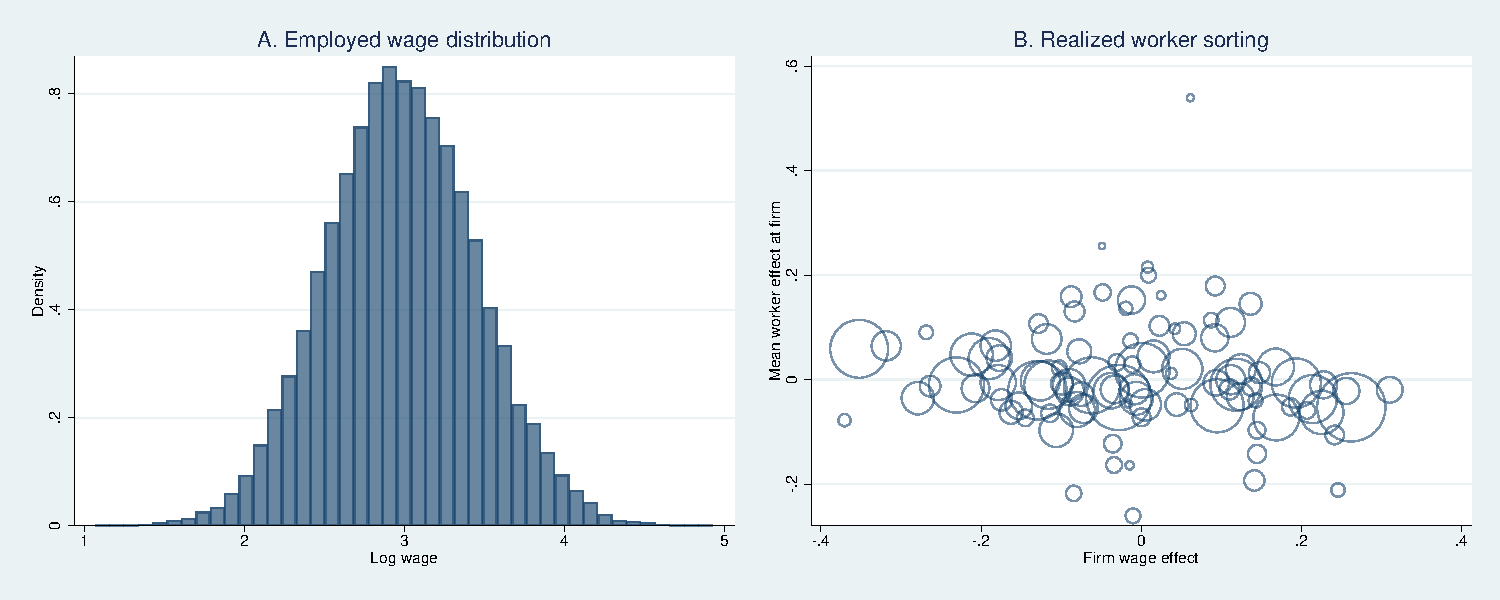
\includegraphics[width=\textwidth]{manual_figures/01_akm.pdf}
\caption{Simple AKM: 3,000 workers, 100 firms, eight years, seed 20260901.
Left: employed log wages. Right: mean worker effect versus firm effect;
marker area reflects employed-observation count. Attraction creates size
heterogeneity. The random design does not impose positive population
sorting, but finite-sample means vary.}
\end{figure}
\FloatBarrier

\clearpage
\subsection{Monthly mobility and Germany-targeted sorting}
\lstinputlisting{manual_examples/02_mobility.do}
\begin{figure}[!htbp]\centering
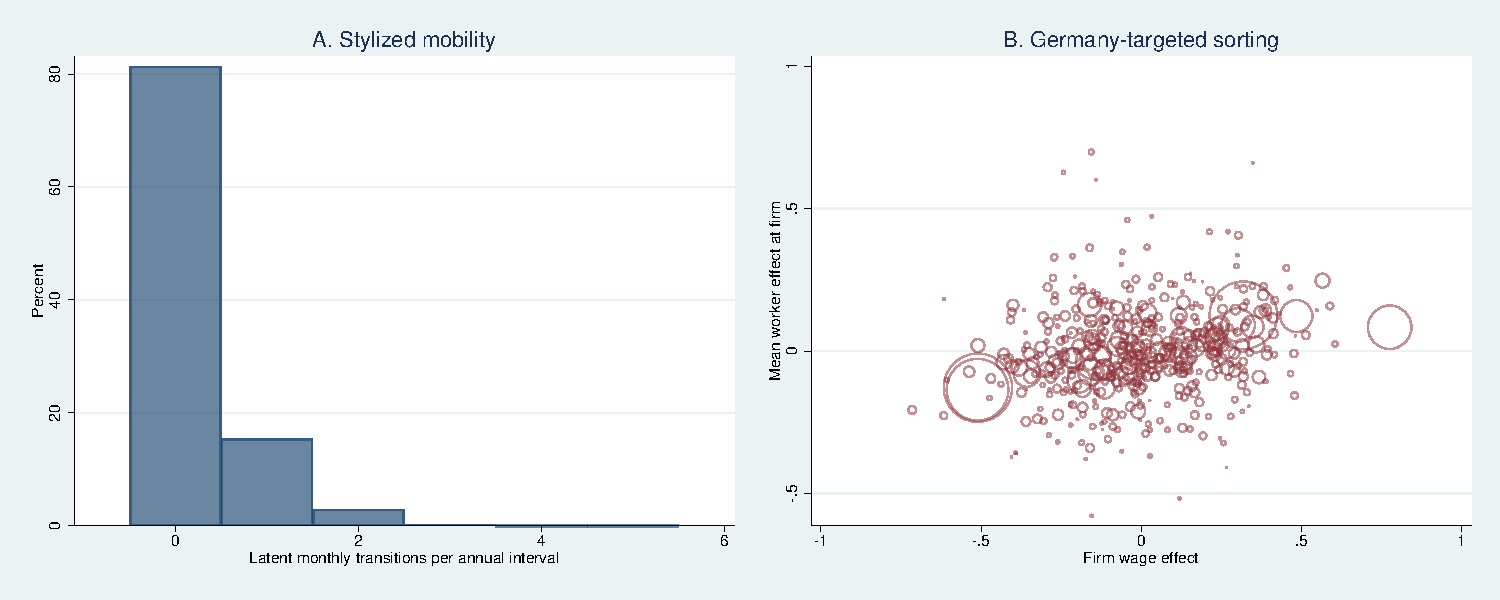
\includegraphics[width=\textwidth]{manual_figures/02_mobility.pdf}
\caption{Two simulations. Left: latent monthly transitions per annual
interval in the stylized engine (3,000 workers, 100 firms, eight years,
seed 20260902), excluding first observations. Right: Germany-targeted
sorting (5,000 workers, 500 firms, eight years, seed 20260903).
Marker area reflects employed observations. Default five-year burn-in
applies to both. The right panel illustrates sorting rather than testing
calibration accuracy in this smaller sample.}
\end{figure}
\FloatBarrier

\clearpage
\subsection{Pay gaps and counterfactual firm schedules}
\lstinputlisting{manual_examples/03_paygap.do}
\begin{figure}[!htbp]\centering
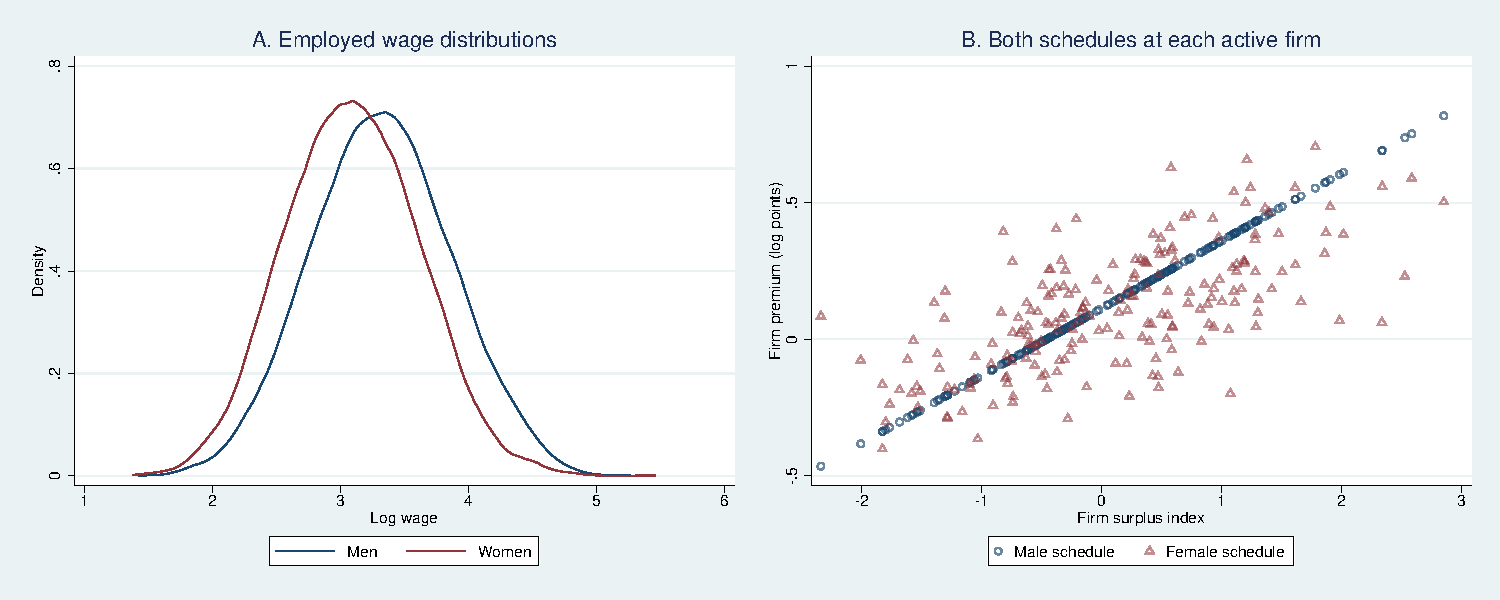
\includegraphics[width=\textwidth]{manual_figures/03_paygap.pdf}
\caption{CCK-inspired data: 5,000 workers, 200 firms, eight annual
observations, five-year burn-in, seed 20260904. Left: smoothed employed
log-wage distributions. Right: one observation per active firm showing both
premium schedules against the same surplus index. The female schedule has
a firm-specific deviation as well as a common-surplus loading. Premiums
use the package normalization.}
\end{figure}
\FloatBarrier

\clearpage
\subsection{BM wage distributions and firm size}
\lstinputlisting[basicstyle=\ttfamily\scriptsize]{manual_examples/04_bm.do}
\enlargethispage{2\baselineskip}
\begin{figure}[!htbp]\centering
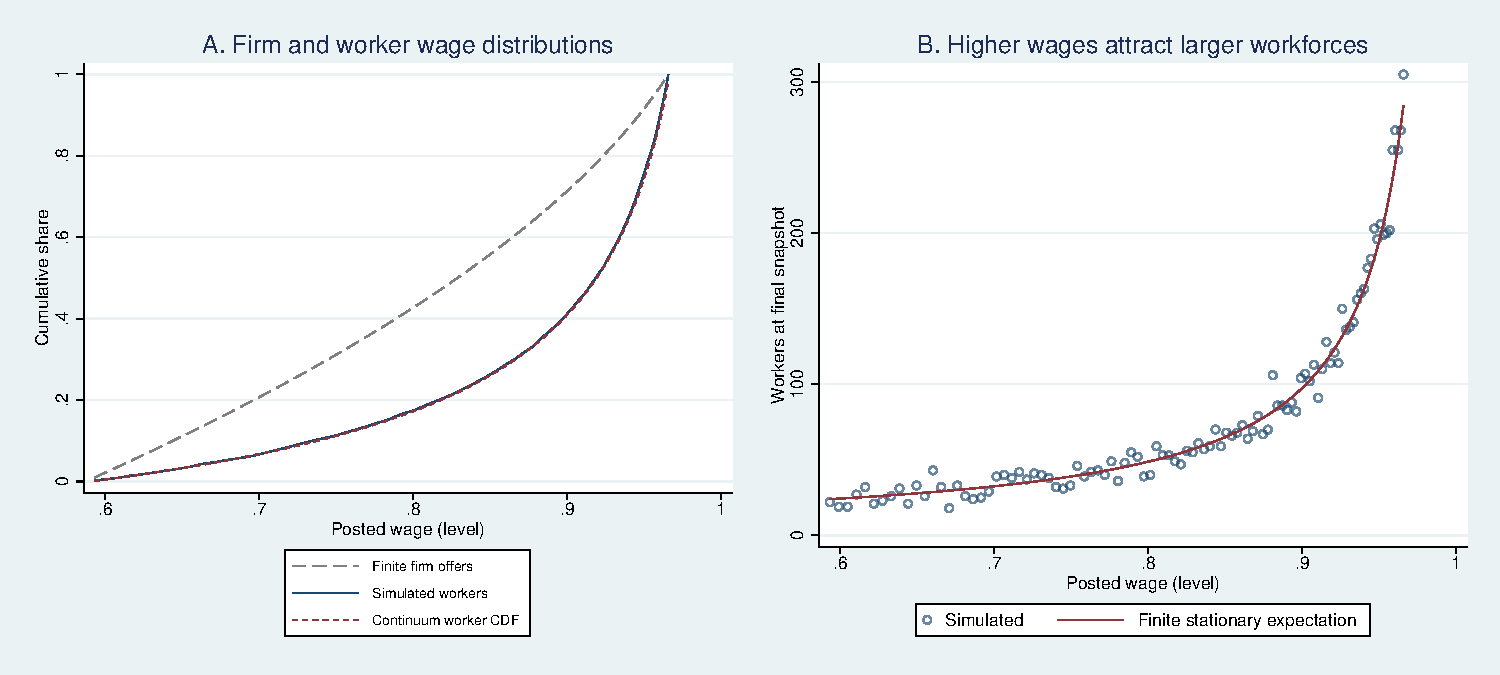
\includegraphics[width=.90\textwidth]{manual_figures/04_bm.pdf}
\caption{Default BM primitives: 10,000 workers, 100 midpoint firms,
five annual observations, stationary start, seed 20260905. Both panels
use the last snapshot. All 100 firms are active in this draw (checked in
code). Lines connect CDF values at finite wage points. Workers concentrate
at higher wages than firm offers, and sizes fluctuate around exact finite
stationary expectations. The continuum worker CDF is a separate benchmark.}
\end{figure}
\FloatBarrier

\clearpage
\subsection{BM worker histories}
\lstinputlisting{manual_examples/05_bm_paths.do}
\begin{figure}[!htbp]\centering
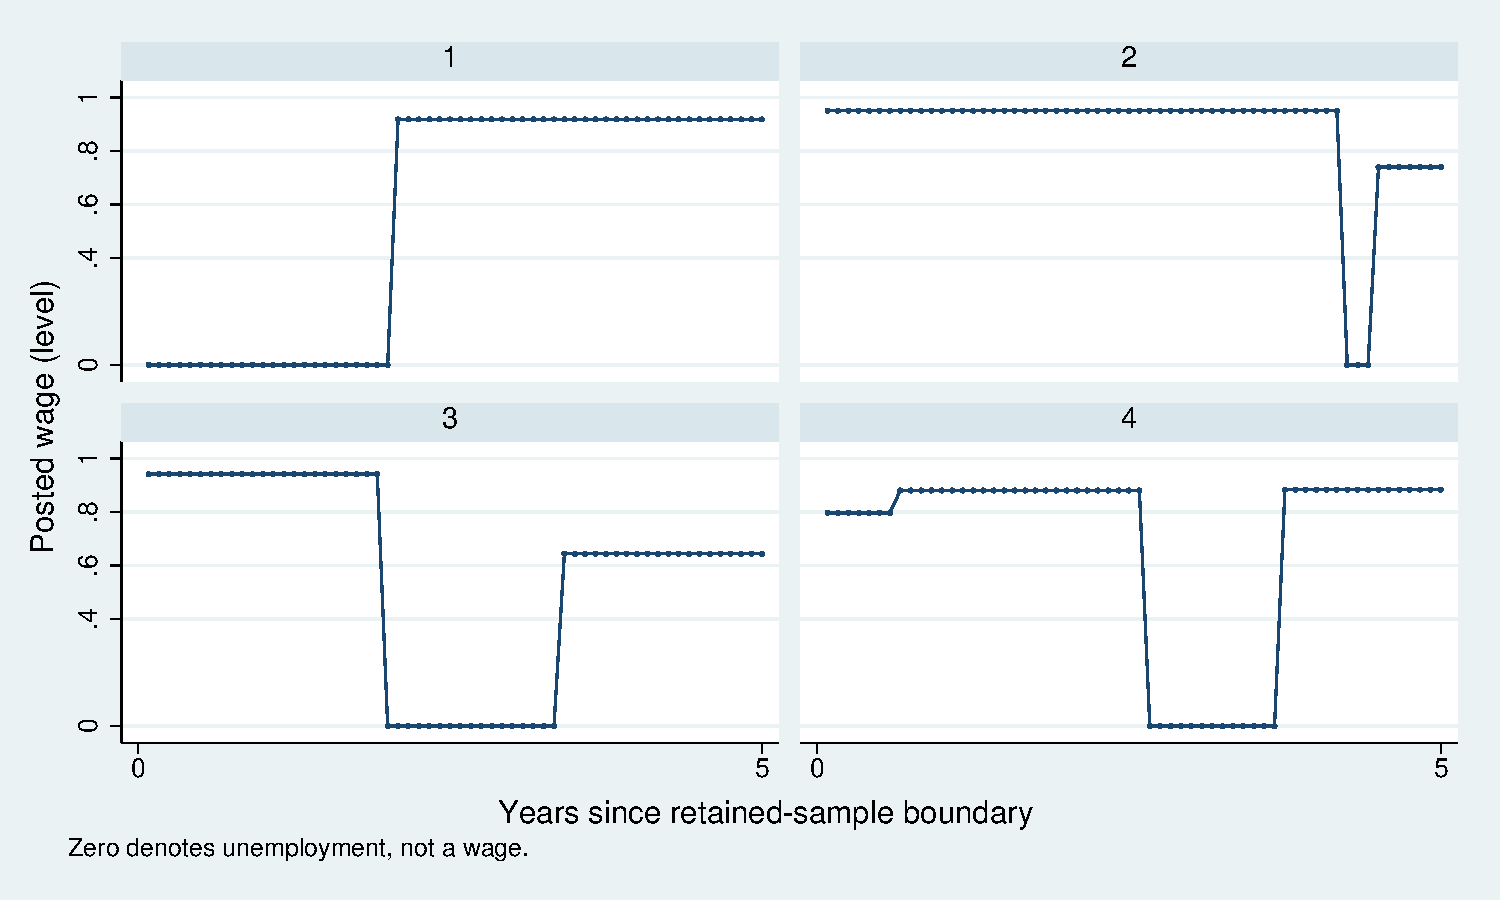
\includegraphics[width=.94\textwidth]{manual_figures/05_bm_paths.pdf}
\caption{First four worker IDs: 300 workers, 100 firms, 60 monthly
snapshots, stationary start, seed 20260906. Zero denotes unemployment only
in the plot; nonemployment wages remain missing in the data. Connected
points are monthly observations, not exact event times. A worker can
separate and re-enter at a lower wage between snapshots even though every
accepted latent EE move is upward.}
\end{figure}
\FloatBarrier

\clearpage
\subsection{BM events versus endpoint probabilities}
\lstinputlisting[basicstyle=\ttfamily\scriptsize]{manual_examples/06_bm_flows.do}
\begin{figure}[!htbp]\centering
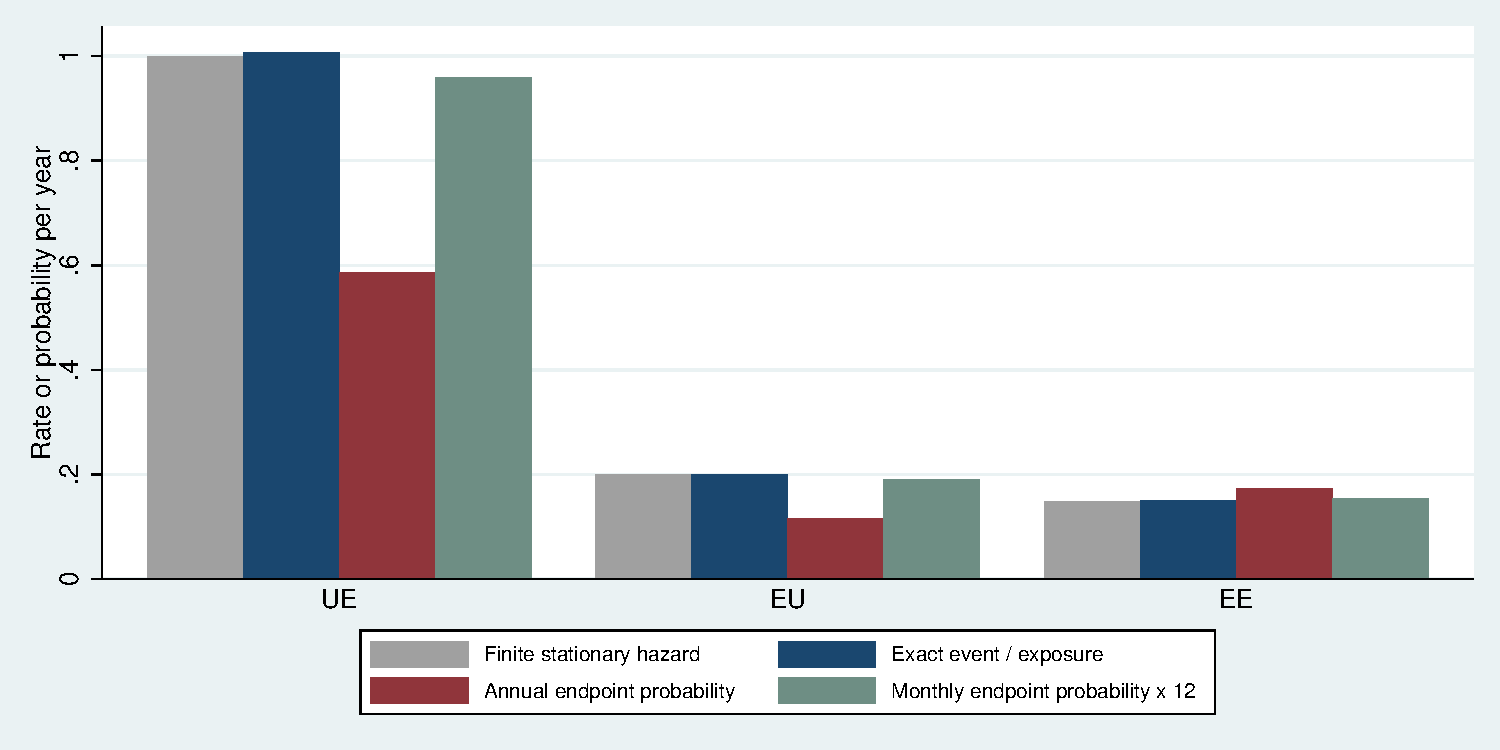
\includegraphics[width=.95\textwidth]{manual_figures/06_bm_flows.pdf}
\caption{BM: 4,000 workers, 100 firms, five years, stationary start,
seed 20260907. Annual and monthly runs use the same continuous history.
Event rates divide accepted transitions by years at risk and agree across
frequencies (asserted). Endpoint probabilities measure different objects.
Multiplying monthly probabilities by 12 is descriptive annualization,
not recovery of a continuous hazard. Observed firm changes can include
intervening unemployment.}\label{fig:flows}
\end{figure}
\FloatBarrier

\clearpage
\subsection{CPV histories: incumbent raises and wage cuts}
\begin{figure}[htbp]\centering
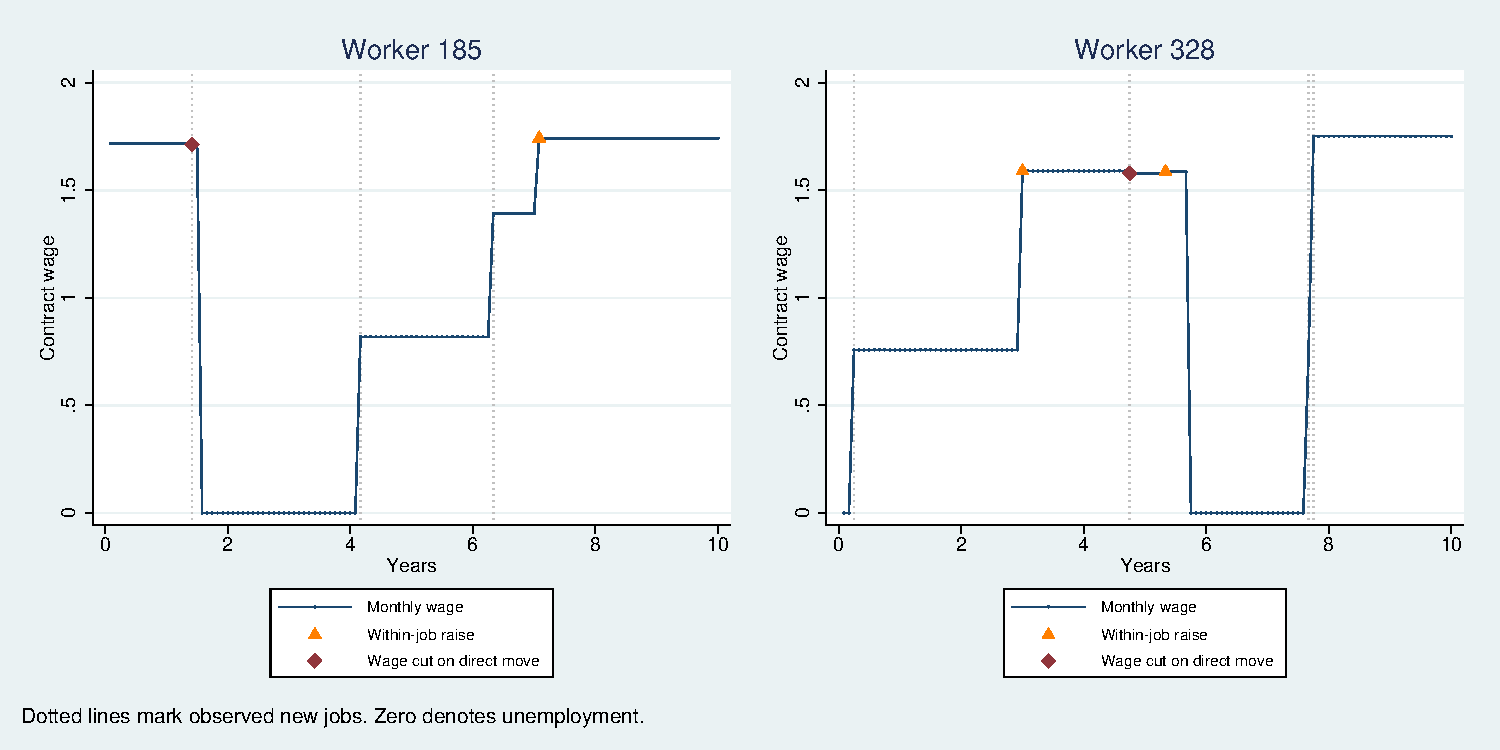
\includegraphics[width=\textwidth]{manual_figures/07_cpv_paths.pdf}
\caption{Two workers selected to illustrate direct-move wage cuts from
1,000 workers, 100 firms and 120 monthly snapshots; seed 20260908,
$\beta=.15$, otherwise simple-preset defaults. Dotted lines identify
observed new jobs, triangles mark within-job raises, and diamonds mark
wage cuts in intervals containing exactly one direct EE and no EU or UE.
These are selected illustrations, not estimates of event frequencies.}
\end{figure}
\lstinputlisting{manual_examples/07_cpv_paths.do}
\FloatBarrier

\subsection{CPV wage dispersion within firms}
\begin{figure}[htbp]\centering
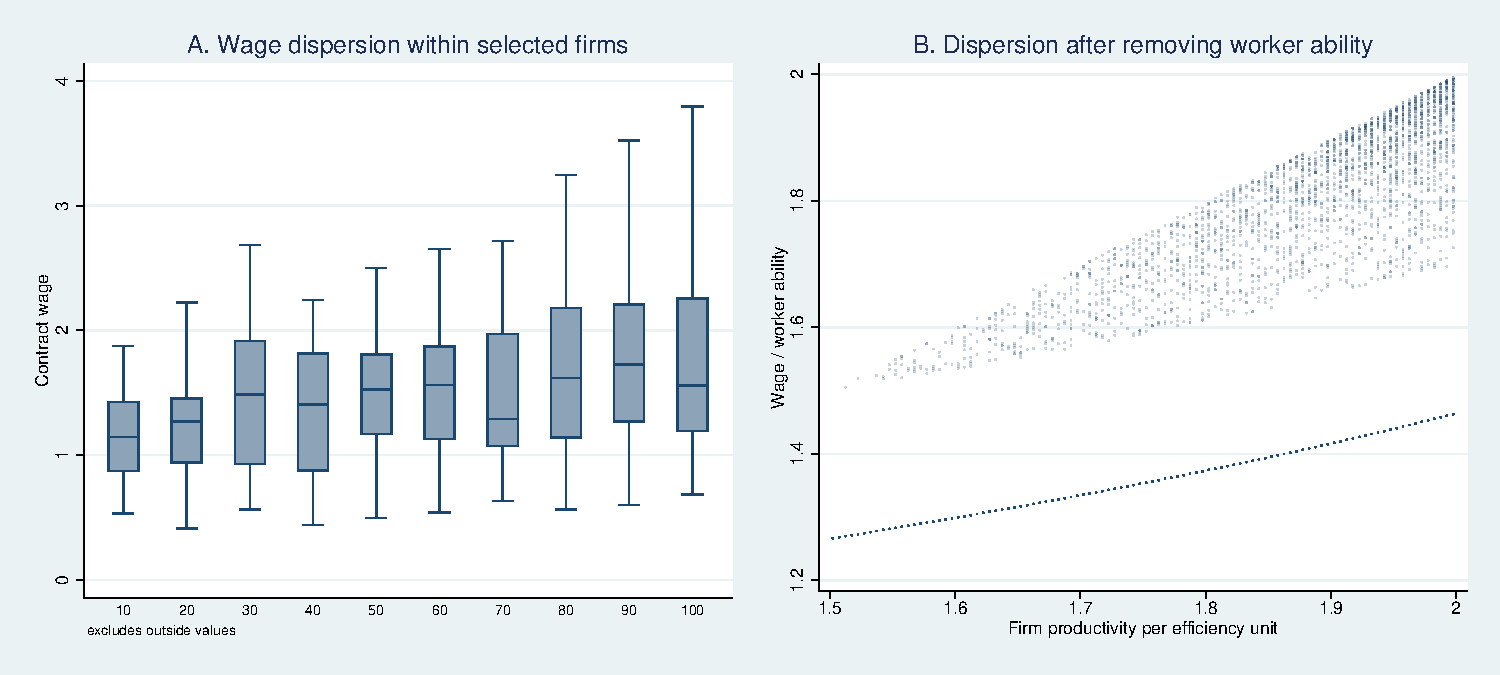
\includegraphics[width=\textwidth]{manual_figures/08_cpv_dispersion.pdf}
\caption{Final annual snapshot of 6,000 workers and 100 firms over three
years, heterogeneous preset, seed 20260909. The left panel shows selected
firms' wage distributions (outside values omitted from the display).
The right panel divides each wage by worker ability: bargaining history
still produces dispersion among workers at the same firm.}
\end{figure}
\lstinputlisting{manual_examples/08_cpv_dispersion.do}
\FloatBarrier

\subsection{Changing bargaining power}
\begin{figure}[htbp]\centering
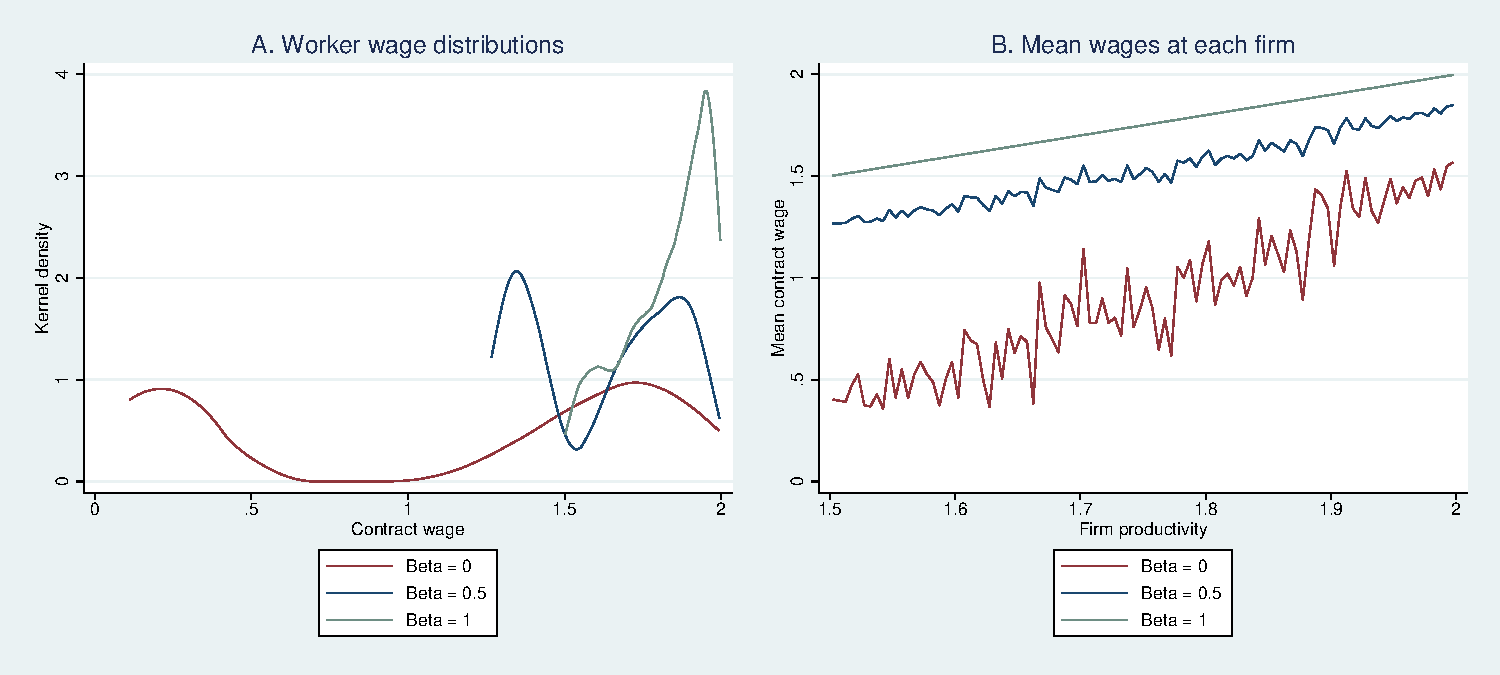
\includegraphics[width=\textwidth]{manual_figures/09_cpv_bargaining.pdf}
\caption{Final snapshot of 4,000 homogeneous workers and 100 firms over
five years, seed 20260910, at three bargaining shares. Firm and employment
paths are held fixed by the seed. Wages change with bargaining power;
at $\beta=1$ workers receive match output and have no incumbent raises.
Kernel curves smooth a discrete finite-firm distribution.}
\end{figure}
\lstinputlisting{manual_examples/09_cpv_bargaining.do}
\FloatBarrier

\subsection{An AKM projection and a mover event study}
\begin{figure}[htbp]\centering
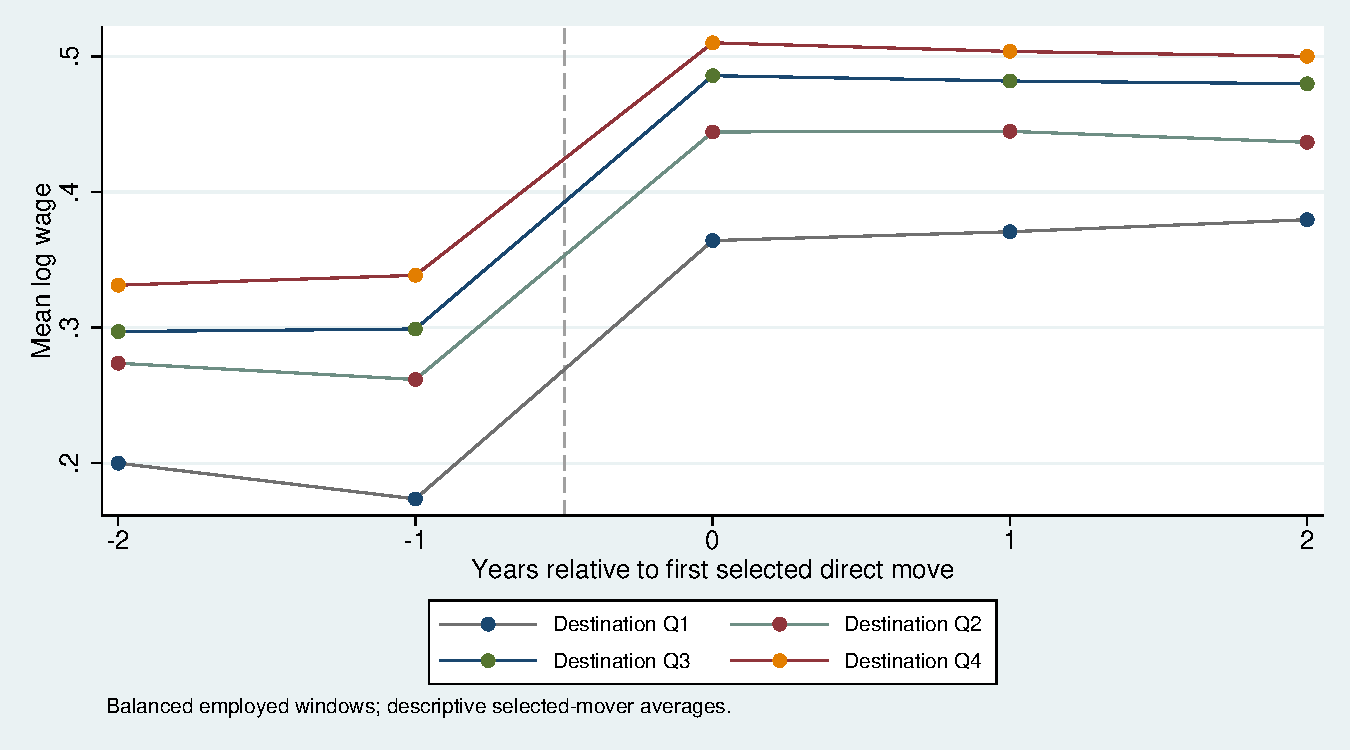
\includegraphics[width=.95\textwidth]{manual_figures/10_cpv_movers.pdf}
\caption{Heterogeneous CPV preset: 5,000 workers, 100 firms, ten annual
observations, seed 20260911. Workers are aligned around their first
selected direct move and must be employed at all five snapshots.
Destination groups are productivity quartiles. These selected-mover
averages are descriptive; they are not causal employer effects.}
\end{figure}
The example uses official \code{areg} to absorb worker effects while
including firm and time indicators. This is an additive projection of
history-dependent wages. Its firm coefficients should not be interpreted
as the primitive productivity levels. There is no population AKM
projection API in this version.
\lstinputlisting{manual_examples/10_cpv_movers.do}
\FloatBarrier


\subsection{BLM interactions and cell distributions}
\begin{figure}[htbp]\centering
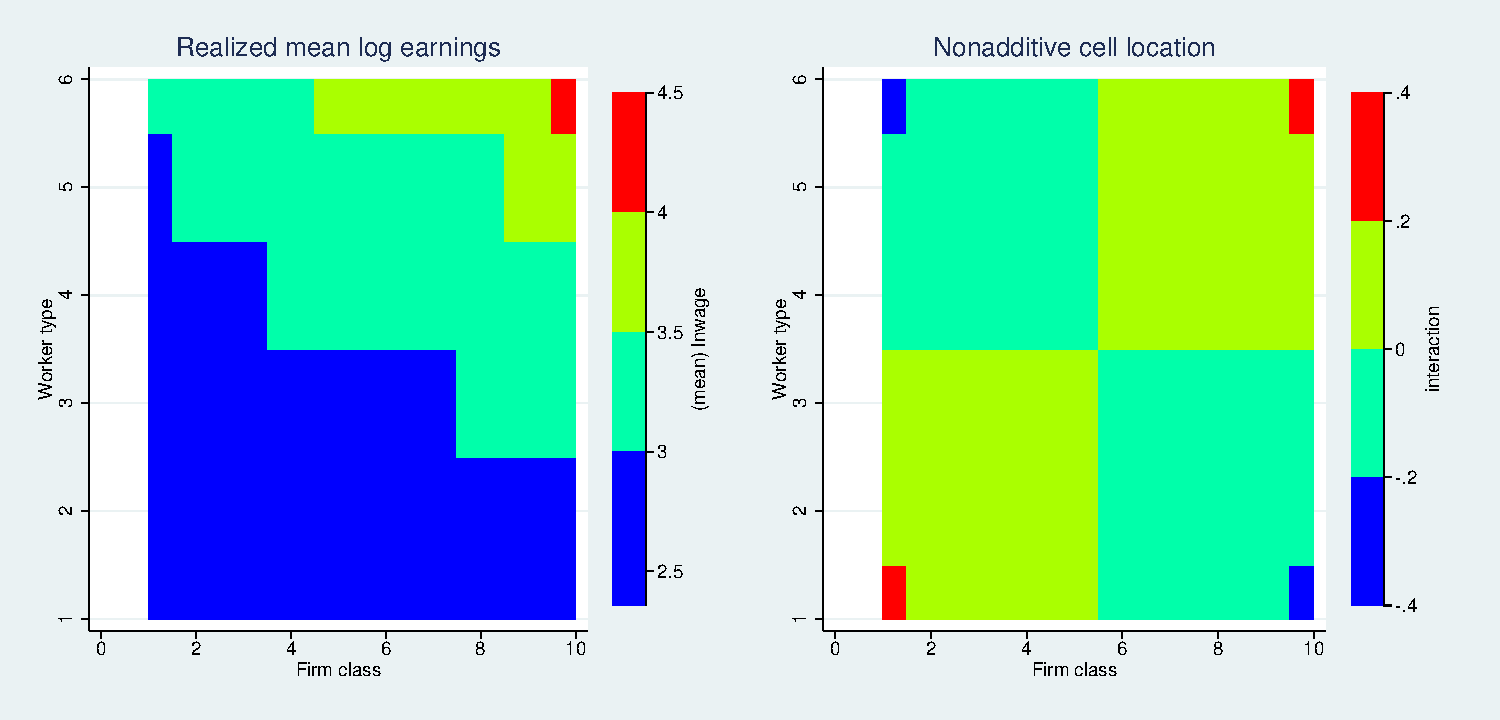
\includegraphics[width=\textwidth]{manual_figures/11_blm_interactions.pdf}
\caption{Static BLM, 6,000 workers and 120 actual firms in ten classes, six
annual snapshots, seed 20260921. Left: realized type/class mean earnings.
Right: nonadditive part of the true cell location after removing unweighted
row and column means. With \code{interaction(0)}, this second panel would be
zero, up to numerical precision. All examples use 20 years of burn-in.}
\end{figure}
\lstinputlisting{manual_examples/11_blm_interactions.do}
\FloatBarrier

\subsection{BLM sorting can have either sign}
\begin{figure}[htbp]\centering
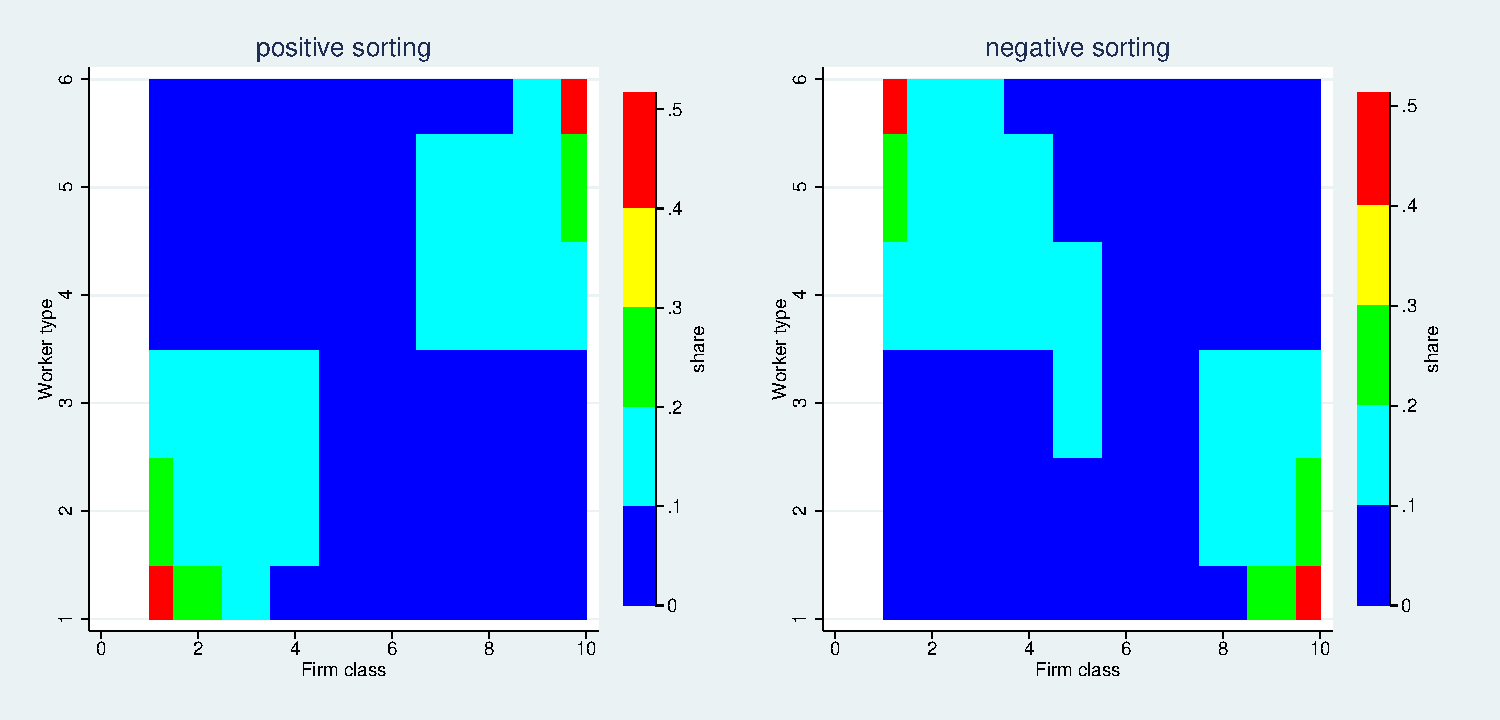
\includegraphics[width=\textwidth]{manual_figures/12_blm_sorting.pdf}
\caption{Static BLM with \code{sorting(1)} and \code{sorting(-1)}, 12,000
workers, 120 actual firms, seed 20260922. Colors show each worker type's
realized employment shares across classes after burn-in and one retained
year. These are employment allocations, distinct from contact probabilities
and the primitive equally weighted class allocation.}
\end{figure}
\lstinputlisting{manual_examples/12_blm_sorting.do}
\FloatBarrier

\subsection{BLM persistent earnings and endogenous moves}
\begin{figure}[htbp]\centering
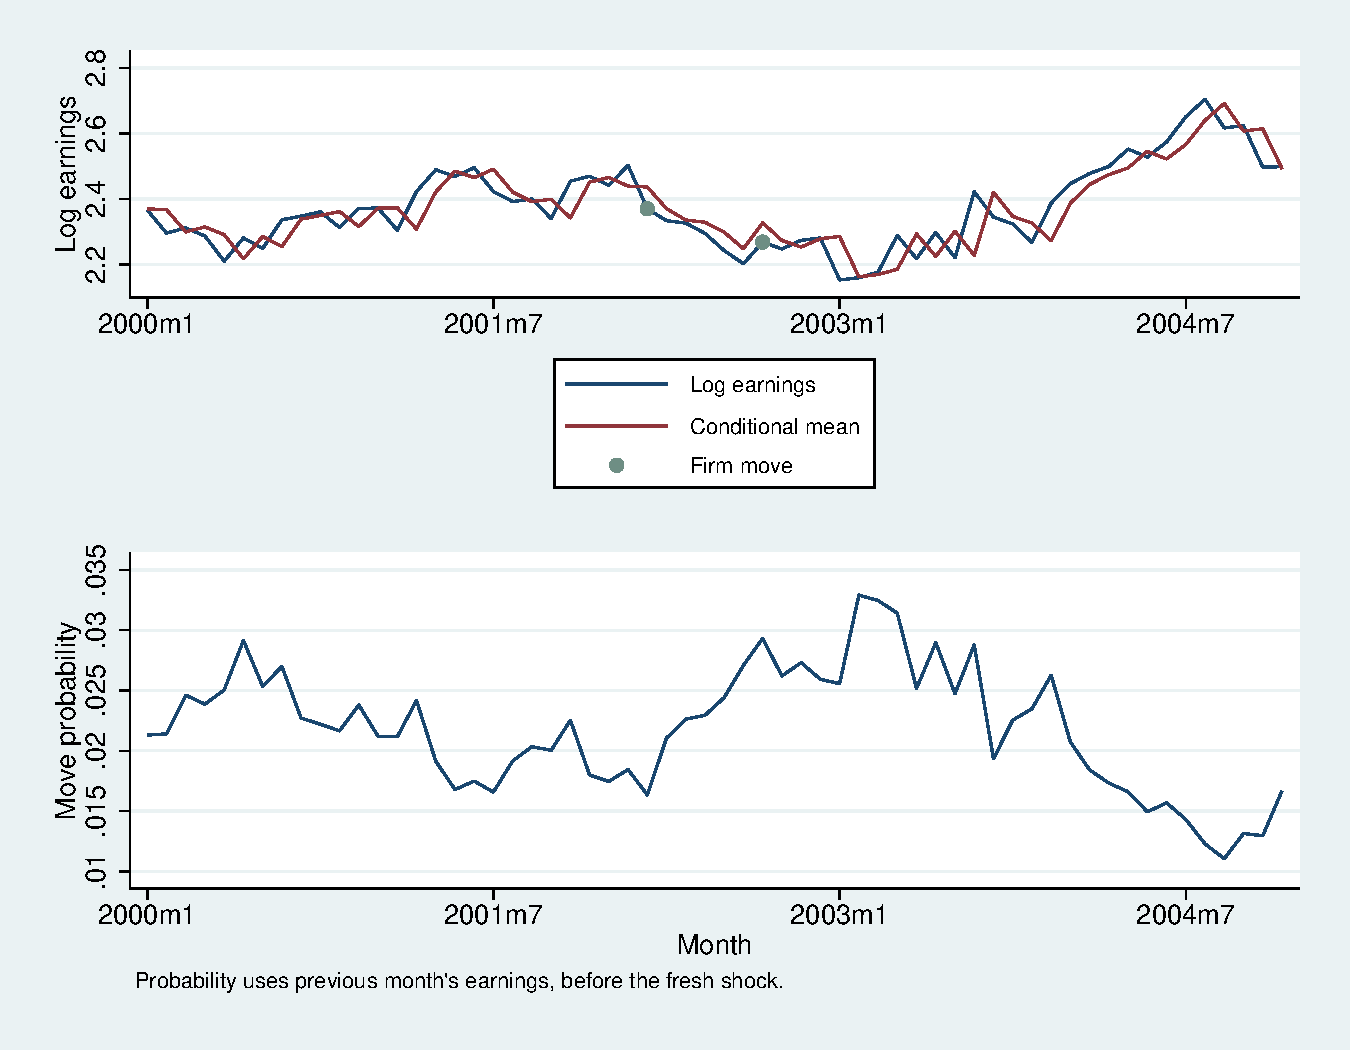
\includegraphics[width=.92\textwidth]{manual_figures/13_blm_dynamics.pdf}
\caption{Dynamic BLM, 1,000 workers, 120 firms, 60 monthly snapshots, seed
20260923. The illustrated worker is the first ID with at least two moves.
The conditional earnings mean includes persistent deviations and any
origin-class move shift. A negative wage-mobility slope raises the next
move probability when the lagged wage is low relative to its cell location.}
\end{figure}
\lstinputlisting{manual_examples/13_blm_dynamics.do}
\FloatBarrier

\subsection{BLM additive projections and mover averages}
\begin{figure}[htbp]\centering
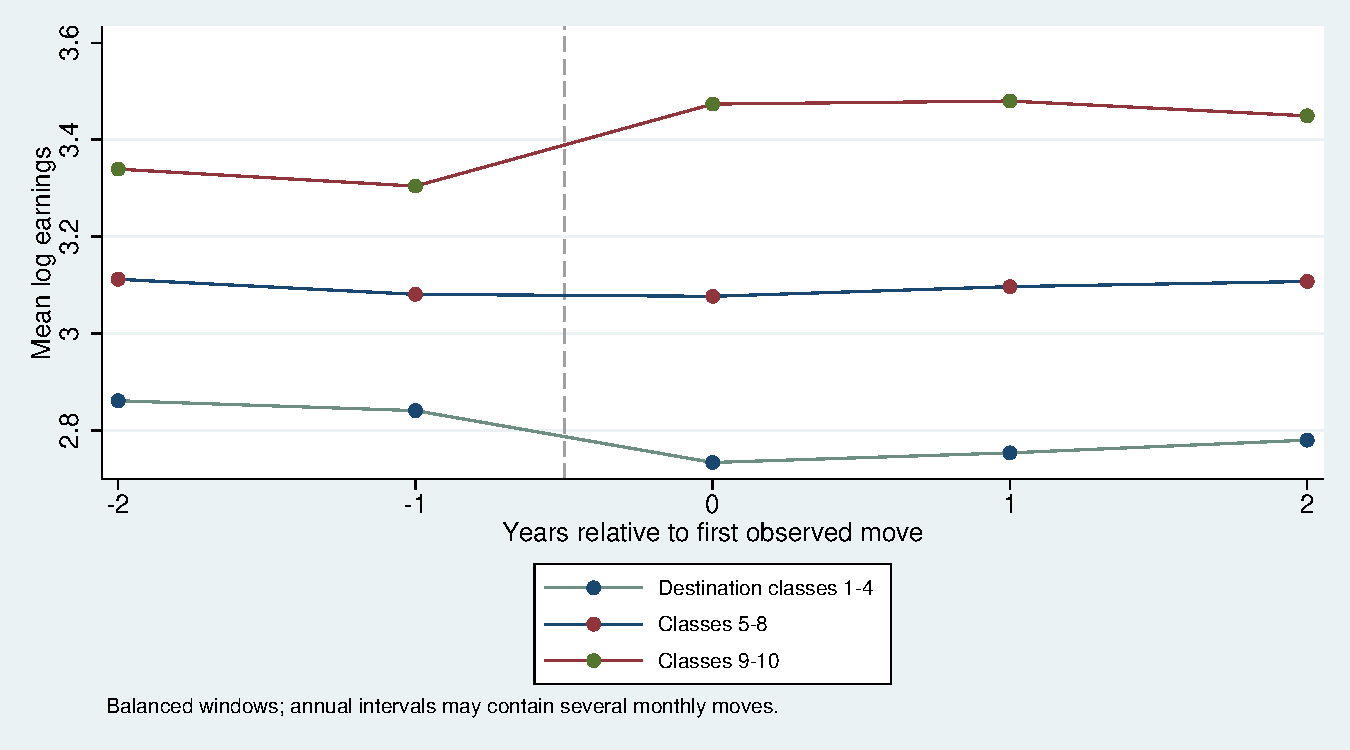
\includegraphics[width=.95\textwidth]{manual_figures/14_blm_movers.pdf}
\caption{Dynamic BLM, 4,000 workers, 80 firms, ten annual snapshots, seed
20260924. Balanced five-year windows around the first observed employer
change are grouped by destination class. Earnings and mobility jointly
select these workers; the lines are descriptive, not causal firm effects.}
\end{figure}
\lstinputlisting{manual_examples/14_blm_movers.do}
The official Stata \code{areg} command estimates an additive projection.
Under interactions, persistent earnings and endogenous mobility, its firm
coefficients need not recover a scalar structural firm effect. Component
connectedness and the package's AKM leave-out diagnostics do not establish
finite-mixture identification.
\FloatBarrier

\subsection{A small estimation exercise}
The simulator does not estimate AKM effects. Official Stata \code{areg}
can fit a small connected example:
\begin{lstlisting}
preserve
fesim, dgp(akmsimple) workers(500) firms(30) periods(6) ///
    seed(24680) truth(none) connectivity(largest) noreport clear
areg lnwage i.workerid i.time if employed, ///
    absorb(firmid) vce(cluster workerid)
restore
\end{lstlisting}
This dummy-variable fit is deliberately small. Estimation normalization is
distinct from the latent-effect normalization. Connectedness alone does
not remove limited-mobility bias in estimated variance components or
establish the assumptions of a particular correction.

\subsection{Three network experiments}
\begin{lstlisting}
preserve
fesim, dgp(akmsimple) network(blocks) workers(400) firms(40) ///
    periods(8) seed(13579) truth(full) ///
    parameters(block_count 4 block_log_bonus 2.1972245773362196) clear
tabulate worker_block_true firm_block_true if employed

fesim, dgp(akmsimple) network(bridges) workers(400) firms(40) ///
    periods(8) seed(246813) burnin(4) truth(full) ///
    parameters(block_count 4 p_eu .02 p_ee .60 p_ue .80) clear
matrix list r(bridges)

fesim, dgp(akmsimple) network(ladder) workers(500) firms(50) ///
    periods(8) seed(161803) truth(full) parameters(p_ee .30) clear
matrix list r(network)
matrix list r(leaveout)
restore
\end{lstlisting}

\clearpage
\appendix
\section{Shared architecture and reproducibility}\label{app:shared}
The ado layer resolves registry and options, validates support and dimensions,
protects caller data/RNG, and dispatches to a Mata handler. The pipeline is:
build population, initialize, discard burn-in, generate retained states,
write the Stata panel, finalize flows, compute diagnostics, attach metadata.

\begin{itemize}
\item \code{fesim_registry.ado} defines parameter names, defaults, bounds,
and provenance.
\item \code{fesim_config.ado} adds cross-parameter restrictions and
canonical serialization.
\item \code{fesim_time.ado} validates dates and interval lengths.
\item Numerical preset records live under \code{calibrations/}.
\end{itemize}
These implementation sources take precedence over historical roadmap
descriptions of future options.

\subsection{Independent random streams}
\code{src/fesim_rng.mata} uses Stata's \code{mt64s} with streams:
101 workers, 102 firms, 103 initial states, 104 mobility events,
105 destinations, 106 wage shocks, 107 observation error,
108 solver/calibration randomization, 109 network design.
It stores full component states in Mata, restores the component before
drawing, and restores the caller's generator and state afterward.
Reserved streams do not imply that every associated feature is public.

An explicit seed preserves the caller sequence. Without a seed, one caller
draw selects a master seed in $[0,2^{31}-1]$. Reporting, truth selection,
and deterministic output do not change economic paths. Invalid
configurations fail before clearing or drawing; later errors restore
the prior dataset and RNG.

\subsection{Time and probability conversion}\label{app:rates}
Let $\Delta$ be output-interval years. Simple AKM and pay-gap convert
annual probabilities to interval probabilities:
\begin{align}
P_{UE}(\Delta)&=1-(1-p_{UE})^\Delta,\\
A(\Delta)&=1-(1-p_{EU}-p_{EE})^\Delta,\\
P_{EU}(\Delta)&=\frac{p_{EU}}{p_{EU}+p_{EE}}A(\Delta),&
P_{EE}(\Delta)&=\frac{p_{EE}}{p_{EU}+p_{EE}}A(\Delta).
\end{align}
When the denominator is zero, both competing probabilities are zero.
At most one transition occurs per interval. This preserves the annual
competing-risk interpretation but does not turn the discrete process into
an exact continuous-time chain allowing repeated within-interval transitions.

Monthly AKM uses $d=1/12$ and annual current-state hazards:
\begin{align}
P_{EU}(d)&=\frac{h_{EU}}{h_{EU}+h_{EE}}
 [1-\exp\{-(h_{EU}+h_{EE})d\}],\\
P_{EE}(d)&=\frac{h_{EE}}{h_{EU}+h_{EE}}
 [1-\exp\{-(h_{EU}+h_{EE})d\}],\\
P_{UE}(d)&=1-\exp(-h_{UE}d).
\end{align}
At most one event occurs per month; hazards update at the next monthly
step. BM instead draws exact continuous waiting times.

\subsection{Output and graph calculation}
AKM handlers retain worker-length state and write period values directly
into worker-major Stata rows without a duplicate full Mata panel.
Complete-worker blocks finalize adjacent-snapshot flows.
BM uses bounded history blocks (Appendix~\ref{app:bmblocks}).
The finalizer computes moments, constructs unique observed matches,
filters if requested, and recomputes moments and diagnostics on retained
workers. Truth moments can exist when latent output columns are suppressed.

Weighting matters: primitive firm distributions weight each firm equally,
whereas many wage/component moments weight employed worker-periods.
Firm-size distributions use active firm-periods. Finite-sample reported
moments therefore need not equal primitive parameters.

\section{Simple AKM implementation}\label{app:akm}
\subsection{Population and wages}
\code{src/fesim_akm_simple.mata} draws independent standard normals
$a_i,z_j,v_j$ and sets
\[
\alpha_i=\sigma_\alpha a_i,\qquad
\psi_j=\sigma_\psi z_j,\qquad
q_j=\frac{\exp(\sigma_qv_j)}{\sum_k\exp(\sigma_qv_k)}.
\]
Weights use max-shifted logs floored at $-700$ to avoid numerical zero
mass. Zero attraction scale gives exact uniform weights. Wage errors
are independent $\epsilon_{it}=\sigma_\epsilon e_{it}$ in \eqref{eq:akm}.
One error draw per worker-period is consumed even if unemployed, preventing
employment counts from shifting wage-stream positions. The wage trend
starts at zero at the first retained observation.

\subsection{Transition matrix and initial state}
Write $a=P_{EU}(\Delta)$, $b_e=P_{EE}(\Delta)$, and $c=P_{UE}(\Delta)$.
For random-network states $0,1,\ldots,J$, with 0 unemployed:
\[
P_{00}=1-c,\quad P_{0j}=cq_j,\quad P_{j0}=a,\quad
P_{jj}=1-a-b_e,\quad P_{jk}=b_e\frac{q_k}{1-q_j}\ (k\ne j).
\]
The stationary initializer solves the actual interval transition rule
(the random case uses a QR-based linear solve and a stationary-residual
check). It does not assign employed workers simply in proportion to $q_j$
when direct moves exclude the current firm. Positive job exits imply a
stationary geometric backward age; if exits are zero, tenure is set to
zero. Network-specific assignment restrictions enter their corresponding
initial-state routines.

Random starts use one-half employment, attraction-weighted firms, and zero
age. All-unemployed starts are draw-free. Burn-in repeats the interval
rule. Simple AKM observes the initialized/burned-in state at the first
retained row; subsequent rows advance one output step.

\subsection{Sampling and spells}
Each step draws one event uniform and one destination uniform per worker.
UE samples entry weights; EE conditions on excluding the origin firm.
EU preserves the completed internal spell count; UE and EE increment it
and reset tenure. Stayers age by one interval. The output finalizer
distinguishes changed spells from changed firm IDs.

\section{Monthly AKM and network implementation}\label{app:empirical}
\subsection{Latent heterogeneity}
Let $a_i,v_i,z_j,\xi_j$ be independent standard normals before mixing.
The worker mobility index is
$m_i=\rho_{z\alpha}a_i+\sqrt{1-\rho_{z\alpha}^2}v_i$, with wage effect
$\sigma_\alpha a_i$. Standard-normal quintile cutoffs map $m_i$ to
$z_i\in\{-2,-1,0,1,2\}/\sqrt2$. Population probabilities are equal;
realized type counts are not forced to match.

Firm quality is the centered, sample-SD-standardized index
$\rho_{q\psi}z_j+\sqrt{1-\rho_{q\psi}^2}\xi_j$, with wage effect
$\sigma_\psi z_j$. Correlation inputs govern latent normals, not exact
realized correlations between discretized types and observed wages.

\subsection{Hazards}
For current firm quality $Q_j$, tenure $\tau$ in years, and unemployment
duration $d_u$ in years:
\begin{align}
\log h_{EU}&=\kappa_{EU}+\beta^w_{EU}z_i+\beta^f_{EU}Q_j+
 \beta^d_{EU}\log(1+\tau),\\
\log h_{EE}&=\kappa_{EE}+\beta^w_{EE}z_i+\beta^f_{EE}Q_j+
 \beta^d_{EE}\log(1+\tau),\\
\log h_{UE}&=\kappa_{UE}+\beta^w_{UE}z_i+
 \beta^d_{UE}\log(1+d_u).
\end{align}
Slopes map to the \code{eu_*}, \code{ee_*}, and \code{ue_*} controls.
Log-sum-exp stabilizes competing probabilities; small-exposure series
avoid cancellation in $1-e^{-x}$. State and durations update monthly.

\subsection{Destination kernels and tables}
For type $z$ set $B_z=\theta_{\rm sort}z+\theta_{\rm quality}$.
UE weights are $q_k\exp(B_zQ_k)$. EE weights from $j$ to $k\ne j$ are
\begin{equation}
q_k\exp\{B_zQ_k+\theta_{\rm up}\max(Q_k-Q_j,0)
                 +\theta_{\rm down}\max(Q_j-Q_k,0)\}.
\end{equation}
A negative \code{theta_down} penalizes downward quality distances.
The code sorts firms by quality and constructs stabilized cumulative
tables by five types, rather than worker-by-firm matrices. Lower/upper
ranges factor into origin terms and destination slopes
$B_z-\theta_{\rm down}$ and $B_z+\theta_{\rm up}$.
Binary searches and range sampling handle origin dependence and exclusion.
Annual/quarterly/monthly snapshots advance 12/3/1 monthly steps, sum latent
transitions, and convert year-valued durations to output units.

\subsection{Calibration and stress designs}
Germany fixes hazard/duration parameters at stylized values and fits only
\code{theta_sort=2.2} after setting three dispersions. The recorded fit
uses five calibration and five disjoint validation seeds, 100,000 workers,
10,000 firms, eight years, and five-year burn-in. Mean covariance is
.0206703882 in calibration and .0200683908 in validation, against .0205
with absolute tolerance .0015. Interactive defaults use a smaller population.

Blocks multiply ordinary destination weights by a same-block factor.
Bridge planning replays strict-block mobility on copied post-burn-in
state and RNG records and chooses distinct eligible workers by independent
network priorities. Economic simulation restarts from original records.
An imposed bridge reuses its EE event's destination uniform and conditions
the kernel on the target block. Later empirical hazards can respond to
that employer: destination-only intervention does not imply invariance
of all future events.

Ladder directions use tied wage-effect percentile ranks and a band.
Direction shares are renormalized over positive ordinary destination
mass, with ordinary weights within direction and the same destination
uniform reused. Initial assignment, UE rules, wages, and the event rule
are not independently redefined by the ladder option.

\section{Pay-gap implementation and decomposition}\label{app:paygap}
\code{src/fesim_paygap.mata} draws groups, group-scaled worker normals,
common firm surplus, independent premium deviations, and separate attraction.
The standardized worker wage primitive determines one of five quintile types.
Conditional on group $g$ and type $z$, destination weights are
\[
\omega_{gj}(z)\propto q_j\exp\{(c_g+d_gz)s_j\},
\]
where $c_g$ and $d_g$ denote \code{group_sort_g} and
\code{worker_sort_g}.
EE excludes the current firm. Group annual probabilities follow
Appendix~\ref{app:rates}. Random starts use one-half employment and
group/type assignment weights before burn-in.

Let $\E_m$ and $\E_f$ average employed male and female observations:
\begin{align}
D&=(\mu_m-\mu_f)+(\E_m\alpha-\E_f\alpha)+F+T+E,\\
F&=\E_m\psi_m-\E_f\psi_f,\quad
T=\E_m(\gamma_m t)-\E_f(\gamma_f t),\quad
E=\E_m\epsilon-\E_f\epsilon.
\end{align}
Here $\gamma_g$ denotes the group-specific wage trend.
Male-reference sorting and schedule terms are
\[
S_m=\E_m\psi_m-\E_f\psi_m,\qquad B_m=\E_f(\psi_m-\psi_f).
\]
Female-reference terms are
\[
S_f=\E_m\psi_f-\E_f\psi_f,\qquad B_f=\E_m(\psi_m-\psi_f).
\]
Both satisfy $F=S_g+B_g$. Symmetric terms are their averages.
The nine returned rows comprise total, intercept, worker composition,
firm total, sorting, premium schedule, time, residual, and adding-up error.
Firm total is a subtotal; do not add it again to sorting and schedule.

CCK targets include male/female log-wage SDs .554/.513, worker SDs
.420/.400, mean premiums .148/.099, premium SDs .247/.213, residual
SDs .143/.125, and worker-premium correlations .167/.152. Targets for
total gap, firm total, sorting, and schedule are .234, .049, .035, .015.
Rounded sorting and schedule targets sum to .050, not .049;
simulated decompositions obey their own exact identity.
Female loading .12567 equals $.590\times.213$, and its deviation SD is
$\sqrt{.213^2-.12567^2}$. The mapping targets selected moments under the
package normalization, not the full CCK estimation procedure.

\section{Canonical Burdett--Mortensen implementation}\label{app:bm}
\subsection{Environment}
Continuum workers and firms each have mass one. Firms have common flow
productivity $p$ and post a permanent wage $w$. Workers receive $b$ while
unemployed and discount at rate $r$. Unemployed/employed offers arrive
at annual Poisson rates $\lambda_u$ and $\lambda_e$, respectively;
jobs are destroyed at rate
$\delta$. Offers sample firms uniformly. Firms maximize steady-state
flow profit, without bargaining, counteroffers, endogenous wage revision,
capacity constraints, or productivity heterogeneity. Unemployed workers
accept wages weakly above reservation wage $R$; employed workers accept
only strictly higher wages.

\subsection{Worker values and reservation}
Let $U$ be unemployment value, $W(w)$ job value, and $F$ the offer CDF
on $[R,\bar w]$. Bellman equations are
\begin{align}
rU&=b+\lambda_u\int_R^{\bar w}[W(x)-U]\,dF(x),\label{eq:U}\\
rW(w)&=w+\delta[U-W(w)]
 +\lambda_e\int_w^{\bar w}[W(x)-W(w)]\,dF(x).\label{eq:W}
\end{align}
Reservation requires $W(R)=U$. Differentiating \eqref{eq:W} gives
\[
W'(w)=\frac{1}{r+\delta+\lambda_e[1-F(w)]}.
\]
Evaluating \eqref{eq:W} at $R$, subtracting \eqref{eq:U}, and
changing integration order yields
\begin{equation}
R=b+(\lambda_u-\lambda_e)S,\qquad
S=\int_R^{\bar w}\frac{1-F(x)}
 {r+\delta+\lambda_e[1-F(x)]}\,dx.\label{eq:reservation}
\end{equation}
Thus $R=b$ when $\lambda_u=\lambda_e$. Imposing that equality
with unequal rates generally violates the worker equations.

\subsection{Stationary workers and firm labor supply}
All support offers are acceptable in unemployment, so
\[
u=\frac{\delta}{\delta+\lambda_u},\qquad e=1-u.
\]
For employed-worker CDF $G$, inflows to jobs below $w$ are
$\lambda_u uF(w)$ and outflows are
$eG(w)\{\delta+\lambda_e[1-F(w)]\}$. Hence
\begin{equation}
G(w)=\frac{\delta F(w)}{\delta+\lambda_e[1-F(w)]}.\label{eq:G}
\end{equation}
Since $G(w)\le F(w)$, workers concentrate at higher wages than offers.
Employment per unit firm mass is
\begin{equation}
\ell(w)=e\frac{dG}{dF}
=\frac{\delta\lambda_u(\delta+\lambda_e)}
 {(\delta+\lambda_u)\{\delta+\lambda_e[1-F(w)]\}^2}.\label{eq:l}
\end{equation}
Profit is $\pi(w)=(p-w)\ell(w)$. Continuum labor supply is not a
simulated integer headcount.

\subsection{Equal-profit equilibrium}
Equating profit at $w$ to profit at the lower support, where $F(R)=0$,
gives
\begin{align}
F(w)&=\frac{\delta+\lambda_e}{\lambda_e}
 \left(1-\sqrt{\frac{p-w}{p-R}}\right),\label{eq:F}\\
\bar w&=p-(p-R)\left(\frac{\delta}{\delta+\lambda_e}\right)^2,\\
w(q)=F^{-1}(q)&=p-(p-R)
 \left(1-\frac{\lambda_e}{\delta+\lambda_e}q\right)^2,\quad 0\le q\le1,
 \label{eq:inverse}\\
\bar\pi&=\frac{\delta\lambda_u}
 {(\delta+\lambda_u)(\delta+\lambda_e)}(p-R).
\end{align}
Profit is constant on support. Wages below $R$ recruit nobody;
wages above $\bar w$ raise wage cost without adding recruitment or
retention advantages over the top support wage.

\subsection{Analytical reservation solution}
Substitution of \eqref{eq:F} into \eqref{eq:reservation} gives
$S=C(p-R)$:
\begin{align}
C&=\frac{2\lambda_e}{(\delta+\lambda_e)^2}
\left[\frac12-\frac{r}{\lambda_e}
 +\frac{r(r+\delta)}{\lambda_e^2}
 \log\left(1+\frac{\lambda_e}{r+\delta}\right)\right],\label{eq:C}\\
R&=\frac{b+(\lambda_u-\lambda_e)Cp}
        {1+(\lambda_u-\lambda_e)C}.\label{eq:R}
\end{align}
This analytical expression is the primary solver. Denominator and
support must satisfy interior and finite-precision checks.
At public defaults, $C\simeq.92842983$, $R\simeq.59022409$,
$\bar w\simeq.96654891$, $u=1/6$, and $\bar\pi\simeq.09756569$.
The continuum accepted EE hazard is
\begin{equation}
h_{EE}^{\infty}
=\lambda_e\int_R^{\bar w}[1-F(w)]\,dG(w)
=\delta\left[\frac{\delta+\lambda_e}{\lambda_e}
 \log\left(1+\frac{\lambda_e}{\delta}\right)-1\right],\label{eq:ee}
\end{equation}
approximately .15077363 at the defaults.

\subsection{Worker values in full truth}
For $q=F(w)$, the implemented values are
\begin{align}
U&=\frac{b+\lambda_u C(p-R)}{r},\\
W(w)&=U+\frac{2(p-R)\lambda_e}{(\delta+\lambda_e)^2}
\left[q+\frac{r}{\lambda_e}
\log\left(1-\frac{\lambda_e q}{r+\delta+\lambda_e}\right)\right].
\label{eq:value}
\end{align}
These are \emph{continuum} values evaluated at discretized wages, not
newly solved Bellman values for the finite offer lottery. The simulation
uses continuum support and strict wage comparisons; finite stationary
employment is computed separately. See \code{src/fesim_bm_output.mata}.

\subsection{Stability and residual checks}
\code{src/fesim_bm.mata} solves afresh on each call. Public numerical
controls are fixed: 1,001 wage-grid points, 4,000 even Simpson intervals,
tolerance $10^{-9}$. There are no public grid options or persistent caches.

For $x=\lambda_e/(r+\delta)<.1$, direct evaluation of the bracket in
\eqref{eq:C} subtracts large nearly equal terms. With $\rho=r/(r+\delta)$
the code uses
\[
\frac{1-\rho}{2}+
\rho\sum_{n=1}^{30}\frac{(-1)^{n+1}x^n}{n+2}.
\]
Otherwise it uses $1/2+\rho\{\log(1+x)/x^2-1/x\}$.
The logarithm helper uses a 40-term alternating series for $|x|<.1$.
For $z=\lambda_e/\delta<.1$, the EE rate uses
\[
h_{EE}^{\infty}
=\delta\sum_{n=1}^{30}\frac{(-1)^{n+1}z^n}{n(n+1)}.
\]
Employment values use the stable logarithm helper. Exact CDF endpoints
are explicitly preserved against division roundoff.

Independent Simpson quadrature over wages checks the reservation equation,
scaling its residual by $\max(1,|b|,|p|,|R|)$. Equal-profit residuals
are scaled by $\max(1,|\bar\pi|)$. Checks require finite support, strict
$0<R<\bar w<p$, positive employment/profit, ordered support, monotone
CDFs in $[0,1]$, and recomputed distribution/labor identities.
Mathematically interior but numerically unresolved inputs can fail explicitly.

\subsection{Finite firms and stationary masses}\label{app:finite}
Default quantiles are $q_j=(j-\tfrac12)/J$ in \eqref{eq:inverse}.
\code{random_firms=1} draws independent uniforms on stream 102 and sorts
them. IDs increase with wage; original draw order breaks quantile ties.
Each firm has contact probability $1/J$.

Let $L_j$ be firm $j$'s share of \emph{all workers}, $L_{<j}$ mass at
strictly lower wages, and $H_j=\#\{k:w_k>w_j\}$. Exact finite flow balance is
\begin{equation}
L_j=\frac{\lambda_u u/J+\lambda_e L_{<j}/J}
          {\delta+\lambda_e H_j/J}.\label{eq:finite}
\end{equation}
The code processes equal-wage groups from low to high, using the same
lower mass and higher-firm count within each group, then updating lower
mass. Tied firms have equal masses and tied offers never induce EE moves.
This linear pass avoids a dense transition matrix.

Masses sum to $e$ and pass stationary-flow residual checks. Expected
headcount is $NL_j$, conditional employed share $L_j/e$, and accepted
finite EE hazard
\[
h_{EE}^J=\lambda_e\frac{\sum_jL_jH_j/J}{e}.
\]
Continuum-scale finite employment/profit are $JL_j$ and $(p-w_j)JL_j$.
They differ from $NL_j$ and from continuum $\ell(w_j)$ and $\bar\pi$.
Finite-scaled profits need not be exactly equal: wages discretize a
continuum equilibrium rather than solve a finite strategic game.

For distinct midpoint wages, offer-CDF discrepancy is $1/(2J)$.
Reported worker-CDF discrepancy compares finite cumulative conditional
masses to \eqref{eq:G} at grid points; it is not Monte Carlo error.
More workers reduce sampling noise, whereas more firms refine discretization.

\subsection{Initial states and burn-in}
Stationary starts draw from $(u,L_1,\ldots,L_J)$. Backward unemployment
age is exponential at rate $\lambda_u$; backward tenure conditional on
firm $j$ is exponential at rate $\delta+\lambda_e H_j/J$.
Rejected offers do not reset tenure and do not enter this accepted-exit
rate. One state and one age uniform per worker use stream 103.

Random starts put one-half probability on unemployment and one-half
uniformly across firms, with zero ages. They require positive burn-in.
All-unemployed starts have zero durations/spells and consume no draws.
Burn-in runs the exact event engine without retaining the ledger, carries
final states/ages forward, and resets retained counters.
Exponential memorylessness permits a fresh wait at the burn-in boundary.
See \code{src/fesim_bm_initial.mata}.

\subsection{Exact event simulation}
For each worker, \code{src/fesim_bm_events.mata} implements:
\begin{enumerate}
\item Set $h=\lambda_u$ if unemployed, or $\lambda_e+\delta$ if employed.
Draw wait $-\log(U)/h$, mapping machine endpoint uniforms into the open
interval so waits are strictly positive.
\item If arrival exceeds the horizon, age the state to the horizon and
stop. Include an event exactly at the right boundary.
\item For an employed event, choose destruction with probability
$\delta/(\lambda_e+\delta)$, otherwise an offer. Equality at the
event-type threshold is an offer.
\item Contact a firm uniformly on any offer. Accept every support offer
while unemployed, and only a strictly higher wage while employed.
Current-firm, lower, and tied offers are recorded rejections.
\item Destruction resets unemployment age. Accepted UE/EE increments
the worker-local spell and resets tenure. Continue from the new state.
\end{enumerate}
Wait/type draws use stream 104; contacts use 105. The combined clock is
equivalent to racing independent Poisson clocks. Workers do not compete
for capacity, so worker-major generation is equivalent to calendar ordering
across workers. Retaining the private ledger cannot alter paths or draws.

\subsection{Observation aggregation}
BM snapshots occur at $\Delta,2\Delta,\ldots,T\Delta$ after the
initialization/burn-in boundary. The zero-time state is not returned.
Intervals are right-closed: $((k-1)\Delta,k\Delta]$. An event at $k\Delta$
affects snapshot $k$ and counts in interval $k$.

\code{src/fesim_bm_aggregate.mata} replays histories without draws, splits
exposure at output boundaries, and counts unemployment/employed offers,
rejections, destructions, accepted UE/EE, all events, and accepted state
transitions. Employment plus unemployment exposure is $\Delta$ per row
up to floating-point tolerance.

Endpoint flags are not event counts. Same-firm re-entry after destruction
changes the spell but not firm ID. Re-entry elsewhere can yield observed
\code{jobtojob=1} despite intervening unemployment. Forward-looking
\code{to_unemp} places a separation flag on the origin row.
For fixed seed, firms, initialization, and total horizon, nested frequencies
preserve final states, events, and exposure. Endpoint probabilities may
differ, as Figure~\ref{fig:flows} illustrates.

\subsection{Bounded blocks and resource guards}\label{app:bmblocks}
\code{src/fesim_bm_handler.mata} initializes the population, simulates
complete worker histories in blocks, aggregates them, and writes directly
into final Stata rows. Persistent event/destination buffers survive block
boundaries and preserve the monolithic worker-major seeded path.
The default block worker count is
\[
\min\left\{10{,}000,\
\max\!\left(1,\left\lfloor\frac{100{,}000}{T}\right\rfloor\right),\
\max\!\left(1,\left\lfloor
\frac{100{,}000}{1+H\max(\lambda_u,\lambda_e+\delta)}
\right\rfloor\right)\right\},
\]
where $T$ is periods and $H=T\Delta$ years. It targets roughly 100,000
rows/events per block; one long worker history can exceed the target.
This is internal, not a public option.

Limits are 10 million workers, one million firms, 100,000 years per
burn-in/retained horizon, and the common observation cap. Each burn-in
and retained stage has a hard 10-million-event budget. Exceeding it causes
rollback rather than truncation. No duplicate full Mata panel or retained
full-population event ledger is stored. Initialization uses $O(N+J)$
storage and $O(N\log J+J)$ work; tie-aware exit rates are linear and
offer acceptance is constant-time after validation.

\subsection{Full truth and diagnostics}\label{app:bmtruth}
Basic truth stores log wage, accepted wage level, and productivity.
No measurement error is added. Full truth adds:
\begin{longtable}{@{}P{0.50\textwidth}P{0.43\textwidth}@{}}
\toprule
Variables & Meaning\\
\midrule
\endhead
\code{reservation_wage_true}, \code{unemployment_value_true} &
Continuum $R,U$, repeated on all rows.\\
\code{employment_value_true}, \code{offer_quantile_true} &
Continuum $W(w_j)$ and accepted-firm offer quantile.\\
\code{expected_firm_mass_true}, \code{expected_firm_share_true} &
Finite $L_j$, $L_j/e$.\\
\code{continuum_employment_true}, \code{finite_scaled_employment_true} &
$\ell(w_j)$, $JL_j$.\\
\code{continuum_profit_true}, \code{finite_scaled_profit_true} &
$(p-w_j)\ell(w_j)$, $(p-w_j)JL_j$.\\
\code{n_eu_true}, \code{n_ee_true}, \code{n_ue_true} &
Accepted counts including the first interval.\\
\code{n_unemployment_offers_true}, \code{n_employed_offers_true},
\code{n_rejected_offers_true} & Primitive offer/rejection counts.\\
\code{n_events_true}, \code{ntransitions_true} &
All events and accepted state transitions.\\
\code{employment_exposure_true}, \code{unemployment_exposure_true} &
Exact years at risk in the interval.\\
\bottomrule
\end{longtable}
Job/firm quantities are missing when unemployed. Counts and exposures
describe intervals regardless of endpoint employment. Internal spell counts
survive unemployment; observed employment-spell IDs follow common missingness.

\code{r(solver)} has 22 rows: six primitives (using \code{discount} for $r$),
surplus coefficient, reservation/upper wages, unemployment/employment,
continuum/finite EE rates, equilibrium profit, unemployment value,
raw/scaled reservation residuals, scaled equal-profit residual,
finite stationary residual, offer/worker CDF errors, finite aggregate
employment error. Its single column is \code{value}.

\code{r(bm_firms)} is 10-by-3 with \code{mean}, \code{min}, \code{max}
across all firms, unweighted. Rows: firm ID, offer quantile, posted wage,
expected mass, expected workers, expected share, continuum employment,
finite-scaled employment, continuum profit, finite-scaled profit.
It is a summary, not a $J$-row dataset.

\code{r(bm_flows)} has rows \code{unemployment_share}, \code{ue},
\code{eu}, \code{ee}, and four columns:
\begin{description}
\item[\code{theory}] $u,\lambda_u,\delta,h_{EE}^J$ in the original finite economy.
\item[\code{event}] Unemployment-time share; UE count over unemployment
years; destruction/EE counts over employed years.
\item[\code{observed}] Endpoint unemployment share and adjacent-endpoint
transition probabilities.
\item[\code{observed_per_year}] Probabilities divided by $\Delta$; the
unemployment-share row is missing. These annualizations are not hazards.
\end{description}
Absent at-risk exposure implies missing event rates.
After \code{connectivity(largest)}, theory/firm summaries still describe
the original unconditioned economy. Realized moments, durations, event
rates, and endpoint probabilities use retained complete-worker histories.
Five temporary count/exposure columns enable this in every truth mode
and are removed before return.

\subsection{Validation scope}
Tests cover equilibrium residuals, equal profit, Bellman identities,
finite masses, ties, singleton firms, deterministic/random grids, replay,
strict acceptance, burn-in convergence, truth/frequency/block invariance,
rollback, and source-only installation. Statistical checks use fixed
seeds and declared tolerances. The candidate inventory contains 68 Stata
test files. Exact macOS Stata/MP 19 qualification receipts and archive hashes
are recorded in the repository qualification guide.

Limit tests approach equal offer rates, small employed offers, rare
destruction, and small positive discounting. Public rates remain positive.
A finite one-firm economy has no accepted EE events even though its
parent continuum has positive EE mobility. Larger $N$ cannot remove
discretization error from fixed small $J$.

Historical benchmark source \code{38eb5bc} reports 100,000 workers over
ten years in 17.943 seconds without truth and 21.526 seconds with full
truth, with peak process RSS about 0.602 and 0.999 GB on that host.
These environment-specific measurements are not guarantees.
Public solve-only/saved-solution interfaces and heterogeneous BM remain
outside the current command.

\section{CPV sequential bargaining implementation}\label{app:cpv}
\subsection{Environment and the source protocol}
Workers have fixed ability $\varepsilon_i>0$; firm $j$ has productivity
$p_j>0$. Output is $\varepsilon_i p_j$, unemployment flow utility is
$\varepsilon_i b$, and utility is linear. The contact rates are
$\lambda_u$ while unemployed and $\lambda_e$ while employed; jobs end
at rate $\delta$ and workers discount at $r$. All firms have contact
weight $a_j=1/J$. A contact with one's employer is a null offer, not
another competitor. Equal-productivity distinct firms can compete over
wages, but never generate a direct employer move between themselves.

The protocol is CPV's original competition followed by bargaining over
worker values. A less productive rival can trigger a raise even if its
full value falls short of the worker's current promised value. Requiring
that rival to beat the current promise would change the model. The share
$\beta$ is imposed, rather than estimated. At $\beta=0$ competition
operates as sequential auctions; at $\beta=1$ the worker receives full
match output and incumbent offers cannot produce further raises.

\subsection{Finite-firm full values and unemployment}
All following quantities are per efficiency unit. Let $U$ be the value of
unemployment, $B=rU$, and $M_j$ the worker's value at firm $j$ when the
current wage equals its entire productivity $p_j$. Thus $M_j$ is the
full-productivity worker benchmark, not a separately computed sum of
worker and firm values. Write $S_j=M_j-U$. An entry contract promises
$U+\beta S_j$, giving
\begin{equation}\label{eq:cpvU}
 B=b+\lambda_u\beta\sum_j a_j S_j.
\end{equation}
At full productivity an incumbent cannot improve the current contract.
A higher-productivity rival $k$ instead delivers $M_j+\beta(M_k-M_j)$.
The worker's Bellman equation therefore implies
\begin{align}
 (r+\delta)S_j
 &=p_j-B+\beta\lambda_e\sum_{p_k>p_j}a_k(S_k-S_j),\\
 (r+\delta+\beta\lambda_e A_j^+)S_j
 &=p_j-B+\beta\lambda_e T_j^+,\label{eq:cpvS}
\end{align}
where $A_j^+=\sum_{p_k>p_j}a_k$ and
$T_j^+=\sum_{p_k>p_j}a_kS_k$. Tails are strictly above the entire
productivity tie group.

The implementation solves this finite system, rather than inserting
continuum wages into a finite contact process. Starting with the most
productive group, express each $S_j=A_j-B C_j$:
\begin{align}
 A_j&=\frac{p_j+\beta\lambda_e\sum_{p_k>p_j}a_kA_k}
 {r+\delta+\beta\lambda_e A_j^+},&
 C_j&=\frac{1+\beta\lambda_e\sum_{p_k>p_j}a_kC_k}
 {r+\delta+\beta\lambda_e A_j^+},\\
 B&=\frac{b+\lambda_u\beta\sum_j a_j A_j}
 {1+\lambda_u\beta\sum_j a_j C_j}.\label{eq:cpvsolve}
\end{align}
Group suffix sums give linear work and storage after sorting. There is
no dense $J$-by-$J$ production solver. Solved surpluses must all be
positive. The scaled residual of each Bellman equation, normalized by
$\max(1,|p_j|,|B|)$, and the unemployment residual normalized by
$\max(1,|B|)$ must be at most $10^{-9}$. Independent small-economy tests
solve the full dense linear system with a $10^{-12}$ comparison bound.

\subsection{The contract state and each offer case}
A contract stores employer $j$ and reference $q$. The reference $q=0$
denotes unemployment, with $S_0=0$. Define the promised surplus
\begin{equation}\label{eq:cpvcontract}
 C(q,j)=\beta S_j+(1-\beta)S_q.
\end{equation}
Upon a contact from firm $k$, the deterministic update is
\begin{equation}
 (j',q')=\begin{cases}
 (j,q),&k=j,\\
 (k,j),&p_k>p_j,\\
 (j,k),&k\ne j,\ p_k\le p_j,\ S_k>S_q,\ \beta<1,\\
 (j,q),&\text{otherwise}.
 \end{cases}
\end{equation}
Only the second case is an EE transition. Only the third is a
renegotiation. Tied firms share the same full surplus, so a different
firm of equal productivity can bring the worker to full surplus.
Reference updates at $\beta=1$ are unnecessary when they change no
value; the stored reference then remains the entry reference or last
employer from a move. Neither null offers nor raises reset job tenure.

\subsection{Recovering wages from promises}
Let $C_k'$ be the promised surplus after the contact update above. While
the current contract is unchanged its wage is constant. Its Bellman
identity yields
\begin{equation}\label{eq:cpvwage}
 w(q,j)=B+(r+\delta)C(q,j)
       -\lambda_e\sum_k a_k\{C_k'-C(q,j)\}.
\end{equation}
Higher rivals contribute
$\beta S_k+(1-\beta)S_j-C(q,j)$.
Lower or equal rivals with $S_k>S_q$ contribute
$(1-\beta)(S_k-S_q)$, except the current employer, whose contribution
is zero. Prefix sums of surpluses and group endpoints evaluate both
sums in constant time; the current employer's atom is explicitly
subtracted from the second sum.

Equation~\eqref{eq:cpvwage} gives $w(j,j)=p_j$ and an increasing wage
in the reference surplus. Entry $q=0$ is the minimum contract wage at a
firm. Every entry wage must be positive; neither negative wages nor
invalid surpluses are clipped. Higher worker value at a new employer
need not mean a higher current wage, because the expected future gain
term can increase. A frozen test verifies a value-improving move with a
current wage cut, and another verifies a raise from a rival below the
current promise.

As $J$ grows, a uniform grid converges to the continuous offer model.
For an interior reference $x$ and employer $y>x$, the independent
continuum check uses CPV's equation (3):
\begin{equation}
 \phi(x,y)=y-(1-\beta)\int_x^y
 \frac{r+\delta+\lambda_e\bar F(z)}
 {r+\delta+\beta\lambda_e\bar F(z)}\,dz.
\end{equation}
For uniform productivity, the integral has an elementary logarithmic
form (and a polynomial limit at $\beta=0$). Tests compare it with
500- and 5,000-firm solutions away from the entry boundary. Finite
self-contact and tied-firm corrections are retained in simulated wages.

\subsection{Worker and firm primitives}
For the simple preset, $\varepsilon_i=1$. Otherwise,
\begin{equation}
 z_i\sim N(0,1),\qquad
 \varepsilon_i=\exp(\sigma z_i-\sigma^2/2),\quad
 \sigma=\text{\code{sd_worker}}.
\end{equation}
This is a population mean-one normalization, not sample
restandardization. Every wage and value is multiplied by
$\varepsilon_i$; production is $\varepsilon_i p_j$. Nonpositive or
nonfinite simulated ability or wages cause a transactional error.
Because contact rates and comparisons are common and per efficiency
unit, changing $\sigma$ leaves the same seeded employment path intact.
In population, ability is independent of employer productivity.

Midpoint firms use $v_j=(j-1/2)/J$ and
$p_j=p_{\min}+(p_{\max}-p_{\min})v_j$. Random firms use sorted
independent uniform quantiles. IDs follow sorted productivity; exact
ties remain ties. The economy does not add free entry, minimum wages,
sector calibration, endogenous ability sorting, amenities, measurement
error, or productivity shocks.

\subsection{Exact finite stationary employment and raises}
Unemployment is $u=\delta/(\delta+\lambda_u)$. If $F$ is cumulative
offer mass through a whole productivity group, stationary balance for
workers at or below that group gives
\begin{equation}
 G(F)=\Pr(p_{\rm employer}\le p\mid E)
 =\frac{\delta F}{\delta+\lambda_e(1-F)}.
\end{equation}
Divide each group increment in $G$ equally among its firms and multiply
by $1-u$ to obtain unconditional masses $m_j$. The exact EE hazard per
employment year is
\begin{equation}
 h_{EE}=\lambda_e\sum_j\frac{m_j}{1-u}A_j^+.
\end{equation}
For an offered productivity group whose first sorted index is $l$,
consider the stationary mass at any eligible incumbent with reference
strictly below that offered productivity. Inflow is a UE into that
incumbent or a move from a lower-productivity employer. Destruction or
a sufficiently good rival removes the worker from this subset. Thus
\begin{equation}
 H_l=\frac{u\lambda_u+\lambda_e\sum_{p_h<p_l}m_h}
 {J\delta+\lambda_e(J-l)}.
\end{equation}
For each offered firm there are $J-l$ eligible incumbents, after
excluding self. When $\beta<1$, the exact raise hazard is
\begin{equation}
 h_R=\frac{\lambda_e}{J(1-u)}
 \sum_{\text{groups }g} |g|(J-l_g)H_{l_g}.
\end{equation}
It is zero at $\beta=1$. These quantities require linear work; a dense
CTMC over all admissible $(j,q)$ states is used only as an independent
tiny-economy test oracle.

\subsection{Stationary contracts and tenure without a dense state solver}
A stationary employed worker's elapsed time since the last UE entry is
$A\sim\operatorname{Exp}(\delta)$: conditional on employment, entry
cohorts survive at the common destruction rate. At time $-A$, sample a
uniform entry employer and set $q=0$. Replay employed contacts at rate
$\lambda_e$ up to zero, conditioning on no intervening destruction.
The final employer, reference and elapsed time since the last direct
move jointly generate the stationary contract and job tenure. Sampling
only an employer and assigning an independent entry wage would fail
this joint-stationarity requirement.

Conditional unemployment, backward unemployment duration is
$\operatorname{Exp}(\lambda_u)$. All initialization draws, including
historical offers, use the initial-state stream. The initial public
spell counter starts at one for an employed worker; unobserved historical
job numbers are not exposed. Random initialization instead uses half
employment, uniform employers, entry contracts and zero ages.
All-unemployed initialization uses zero ages and no initial-state draws.

Independent tests construct the finite contract-state generator and
solve its stationary distribution. For each employer, uniformization of
the within-employer subgenerator gives joint contract masses with
job tenure exceeding two years. Two disjoint 100,000-worker fixed-seed
samples must satisfy predeclared absolute bounds of .005 for state
masses and .004 for the contract--tenure tail. Long burn-in and returned
flow tests use separate seeds.

\subsection{Event clock, observation, storage and failures}
The total primitive event rate is $\lambda_u$ while unemployed and
$\delta+\lambda_e$ while employed. Waiting times are exponential. An
employed event is destruction with probability
$\delta/(\delta+\lambda_e)$; otherwise it is a uniform firm contact.
Unemployed contacts enter a job, since every firm was validated viable.
Self and rejected contacts remain primitive events. Destruction records
an EU; entry records a UE; only an upward employer change records EE.

Snapshots are taken at $\Delta,2\Delta,\ldots,T\Delta$. An event exactly
at the endpoint belongs to that interval and its resulting state is
observed. A waiting time drawn beyond one endpoint is carried into the
next interval. No redraw occurs just because output frequency changes.
Exact E/U exposure accumulates along each segment in years. Observed
flow flags follow the common endpoint rules, and public first-row
\code{ntransitions} is missing even though full truth records that first
interval's latent counts. A same-firm return creates a new spell and
latent EU/UE without an observed employer-to-employer flag.

Uniform draws are buffered in blocks of 4,096 per component. Buffers
survive worker and processing-block boundaries. Ability, firm primitives,
initial states, event clocks and destinations use the established
separate RNG streams. Fixed-seed none/basic/full output, ability changes,
block sizes and nested frequencies are checked for path invariance.

The public writer uses at most
$\min\{10{,}000,\max(1,\lfloor100{,}000/T\rfloor)\}$ workers per block;
a single worker's full requested history is the unavoidable minimum.
It stores no population-wide event ledger. Bounds are ten million
workers, one million firms, 2,147,483,647 requested rows, and 100,000
years for each horizon. Initialization permits at most ten million historical employed offers;
burn-in and retained simulation each have a ten-million primitive-event budget. Failure restores caller
data and RNG, including errors after random firm construction. Nonfinite lifetime values
or ability-scaled productivity/value bounds are rejected under every truth mode.

\subsection{Truth and result interpretation}
Basic truth reports five structural objects:
\begin{center}\small
\begin{tabular}{@{}ll@{}}
\toprule
Variable & Meaning\\
\midrule
\code{lnwage_true} & Log contract wage\\
\code{contract_wage_true} & Contract wage level\\
\code{worker_ability_true} & Fixed worker efficiency units\\
\code{firm_productivity_true} & Firm productivity per efficiency unit\\
\code{match_productivity_true} & Worker ability times firm productivity\\
\bottomrule
\end{tabular}\end{center}
Ability is defined even while unemployed; job attributes are missing then. Full truth adds the reference firm,
reference surplus and value, unemployment value, employment value,
full-productivity match benchmark, and exact interval EU/EE/UE, offers,
rejections, events, transitions, renegotiations and exposure. Reference
firm zero means unemployment; reference value is then the worker's $U$.
All reported values scale with worker ability.

\code{r(solver)} has 17 named rows: primitives and realized firm support,
unemployment value and shares, finite EE and raise hazards, Bellman
residual, minimum surplus and entry wage, and firm count.
\code{r(cpv_firms)} summarizes eight firm objects by mean/minimum/maximum:
ID, quantile, productivity, full surplus, entry wage, expected mass,
expected workers and conditional employment share. No large public
Stata matrix of all firms is required.

\code{r(cpv_flows)} has rows for unemployment share, UE, EU, EE and
renegotiation, and columns for theory, event/exposure, observed endpoint
probability and the descriptive endpoint probability per year.
Renegotiation has no endpoint-transition analogue, so its last two
columns are missing. With \code{connectivity(largest)}, theoretical
objects and generated-event counts describe the original economy;
realized rates, moments and durations are recomputed for returned workers.
Six temporary count/exposure variables are removed before return under
every truth setting. Structural truth is not labeled as AKM firm truth.

\subsection{Equation audit and qualification boundary}
The source audit uses the November 2005 author revision linked from
Jean-Marc Robin's publications page, SHA256 prefix
\code{f7e51c74dbd34914}. Rendered PDF pages 9--11 (printed 7--9) establish
the bargaining cases, equation (3), beta limits and wage cuts. Its equation
(4) visibly prints $p_{\inf}$ as the first term although it equates the
expression with equation (3), which uses employer productivity $p$.
This apparent typo is not copied: entry wages follow
Equation~\eqref{eq:cpvwage}. The exact publisher PDF has not been verified;
version-specific source claims retain that qualification. Full source
identity, URL and evidence are in \code{docs/cpv-derivation.md}.

The finite solver, continuous-time simulator and examples implement the
canonical mechanisms with declared stylized primitives. They do not
replicate empirical estimates or calibrate sector and skill groups.
Qualification is for the tested macOS Stata/MP 19 environment. A release
tag, publication and broader platforms remain separate decisions.


\section{BLM finite-type forward simulation}\label{app:blm}
\subsection{Scientific scope and audited versions}
The published reference is Bonhomme, Lamadon and Manresa (2019) \cite{blm}.
The implementation audit uses the IFAU 2017 working paper, PDF pages 10--11
(printed pages 8--9), Assumptions 1 and 2 and equations (1)--(2), and the author
supplement, Section S1.2--S1.3. The main published PDF was unavailable during
the bounded audit; equivalence between that PDF and the working-paper version
is not assumed. \code{docs/blm.md} records URLs, version hashes, code locators
and the mapping from source restrictions to implementation choices.

The static source restriction makes mobility independent of wage history given
type and class/history controls, and requires serial independence of movers'
next earnings conditional on current type and destination. Our static Gaussian
specialization is stronger: every monthly earnings draw, for movers and
stayers, is independent conditional on its cell. The dynamic restriction permits
mobility to depend on current earnings and makes next earnings first-order in
current earnings, worker type, origin/destination class and move status.
Our monthly process satisfies these restrictions by construction. Its Gaussian
shape, score recipes, time-homogeneous tables, scalar defaults, event clock and
initializer are package choices. There are no unemployment or covariate states,
firm-level idiosyncratic effects, estimated mixture parameters, or empirical
calibration targets.

\subsection{Finite populations, probabilities and score normalization}
Choose $N$ workers, $J$ actual firms, $L$ worker types and $K$ firm classes.
Normalize strictly positive input weights to $p_l$ and $q_k$. Each class gets
one actual firm. Allocate the remaining $J-K$ by largest remainders:
\[
 b_k=(J-K)q_k,\qquad n_k=1+\lfloor b_k\rfloor+d_k,
 \qquad \sum_k n_k=J,
\]
where the $d_k\in\{0,1\}$ select the largest fractional remainders, with ties
resolved by lower class index. Actual IDs form contiguous class ranges.
Normalized class weights $q_k$ and realized class shares $n_k/J$ are distinct
when allocation rounds. Worker types are independent categorical draws from
$p$, with no constraint on their realized finite counts.

For $D>1$ define raw normal midpoint scores
$a_d=\Phi^{-1}((d-1/2)/D)$. Given probabilities $w_d$, use
\[
 z_d=\frac{a_d-\sum_e w_e a_e}
 {\sqrt{\sum_e w_e(a_e-\sum_f w_f a_f)^2}}.
\]
Use $w=p$ for worker scores $x_l$ and $w=n/J$ for class scores $z_k$.
For a singleton the score is zero. Weights are scaled by their maximum before
normalizing to avoid overflow. Numerically unresolvable positive weights or
score variance fail validation; they are not silently replaced.
Default cell locations and scales are
\[
 \mu_{lk}=\mu+\sigma_w x_l+\sigma_f z_k+\gamma x_lz_k,
 \qquad s_{lk}=\sigma_e.
\]
These recipes define cell locations, not necessarily unconditional means in the
dynamic economy. Full input matrices can replace each recipe. Additivity means
all cross-differences of $\mu_{lk}$ vanish; setting $\gamma=0$ achieves this
for the scalar recipe without forcing homogeneous wage distributions.

\subsection{Monthly timing and endogenous mobility}
State just before month $m$ is $(l,j,k,y)$, with permanent type $l$, actual firm
$j$ in class $k$ and current log earnings $y$. Let $\lambda_{lk}\geq0$ be the
annual baseline move intensity and $g_{lk}$ its wage slope. First compute
\begin{equation}
 h_{lk}(y)=\lambda_{lk}\exp[g_{lk}(y-\mu_{lk})],\qquad
 P_{lk}(y)=1-\exp[-h_{lk}(y)/12].
\label{eq:blmmove}
\end{equation}
A uniform draw below $P$ triggers an actual-firm move. There is at most one
move per internal month. This is a discrete monthly transition specification,
not an exact continuous-time process with a frozen intensity. A zero rate, or
$J=1$, implies zero move probability regardless of earnings. The destination
draw precedes the new Gaussian wage shock, so that shock cannot cause the same
month's move. Wage dependence operates through the preceding month's earnings.

If $D_{lkh}$ is an input destination mass, normalize it row-wise first.
The scalar recipe is proportional to
\[
 D_{lkh}\ \propto\ n_h\exp(s x_l z_h),
\]
independent of origin $k$ before excluding the current employer. Remove its
per-firm mass, then normalize:
\[
 \widetilde D_{lkh}=D_{lkh}\left(1-\frac{\mathbf1\{h=k\}}{n_k}\right),
 \qquad Q_{lkh}=\frac{\widetilde D_{lkh}}{\sum_a\widetilde D_{lka}}.
\]
The conditional probability of a particular eligible firm in class $h$ is
$Q_{lkh}/(n_h-\mathbf1\{h=k\})$. One uniform draw selects both class and
eligible actual firm by partitioning the corresponding cumulative interval.
Within-origin-class selection skips the old firm ID. A row with no eligible
mass is permitted only when its rate is zero or the economy has one firm.
Conditional rows for impossible moves remain zero. Nonuniform class counts,
within-class moves and self-exclusion therefore affect realized destinations.

\subsection{Earnings transition and interpretation of scales}
Let $M\in\{0,1\}$ indicate a move and $h$ be the selected next class, with
$h=k$ if there is no move. Convert annual $\rho_{lh}\in[0,1)$ into monthly
$\phi_{lh}=\rho_{lh}^{1/12}$. Draw $e\sim N(0,1)$ independently after mobility:
\begin{align}
 c &= \mu_{lh}+\phi_{lh}(y-\mu_{lk})+M C_{lkh},\\
 v &=s_{lh}\sqrt{(1-\phi_{lh})(1+\phi_{lh})},\\
 y'&=c+ve.
\label{eq:blmwage}
\end{align}
Persistence and innovation scale use the destination cell; the carried residual
is centered at the origin cell. The scalar shift is
$C_{lkh}=o(z_k-z_h)$. Within-class shifts are zero for that recipe, although a
full shift table can specify a nonzero shift on within-class moves. Shifts are
applied only when actual firms change. In a fixed cell without moves,
$s_{lk}$ is the stationary earnings SD. With changing cells, selection and
shifts, it need not equal the realized cell SD or innovation SD. A zero scale
is allowed and gives a deterministic conditional wage transition.

Static mode sets $\phi=g=C=0$ exactly. Dynamic mode with all these values zero
uses identical operations and random draws, giving identical static histories.
Annual persistence approaching one closely enough that the monthly value rounds
to one is rejected, rather than silently generating zero innovation variance.

\subsection{Initialization, burn-in, observation and spells}
Random initialization draws a permanent type, a uniform actual firm and
$y_0=\mu_{lk}+s_{lk}e_0$ independently, sets tenure to zero and spell ID to one.
It then advances the same monthly process through burn-in. The default is
240 months; any nonnegative burn-in in years is allowed if it lies on a monthly
grid. This is not an exact stationary initializer. Slow mixing, zero moves and
extreme persistence may retain initialization effects after the default burn-in.

The first retained observation follows one complete requested output interval
after burn-in. Annual, quarterly and monthly output advances 12, 3 and 1 steps;
the endpoint employer and last monthly earnings are recorded, with no average
wage aggregation. Retained paths are identical at shared endpoints for equal
burn-in and total horizons. A move resets monthly tenure to zero and increments
the worker's spell ID. A stayer adds one month; output tenure is divided by
months per output period. Spell numbering includes burn-in history. Counts reset
after burn-in and at every retained interval. Common \code{ntransitions} retains
its first-row missing convention, while \code{n_ee_true} includes the first
retained interval. A return to the previous observed employer can produce
\code{jobtojob=0} alongside positive latent counts and a changed spell.

\subsection{Random streams, storage, numerical guards and provenance}
Streams are worker types 101, initial states 103, mobility events 104,
destinations 105 and wage shocks 106. Initial-state uniforms for all workers
precede their initial normal draws. Every worker-month consumes one event
uniform, one destination uniform and one normal draw, even for impossible moves
or zero innovations, including burn-in. Three-column buffers of 4,096 draws
persist across worker blocks. Worker-major simulation makes output frequency,
truth level and block size irrelevant to the underlying path at matched horizons.

The writer targets 100,000 output rows per block and at most 10,000 workers,
allowing one larger worker history when necessary. It stores no complete
population history beyond the final Stata dataset and the initial population.
Guards limit total output to 2,147,483,647 rows and generated work to one billion
worker-months, including burn-in. Stata edition and memory limits may bind first.

Destination utilities use max-shifted exponentials. Mobility probabilities use
log intensity and stable small-probability arithmetic; underflow and saturation
map to floating-point zero and one. Invalid tables, nonfinite derived wages or
summaries, and exhausted numerical range fail explicitly. Validation precedes
mutation; later failures restore the caller's data and RNG. Exact-source tests
cover both failure paths, caller-owned matrix preservation and large-grid
serialization. Cell moments use Welford updates and are recomputed after
component filtering. Model tables remain those of the generated finite economy.

The resolved model is serialized in fixed table order, dimensions and row-major
values with 17 significant decimal digits. Dataset characteristics hold chunks
of at most 30,000 characters and a count; no values are truncated. The simulation
loads the resolved tables directly, avoiding a second normalization that could
change last-bit destination thresholds. Stata's 32-bit \code{hash1()} supplies a
short fingerprint, which is neither a unique model ID nor an integrity guarantee.

\subsection{Author-model fixtures and identification boundary}
The pinned author repository contains \code{R/m2-mixt.r} and \code{R/m4-mixt.R}.
These generate conditional two- and four-period stayer/mover samples, including
worker-type probabilities conditional on origin/destination classes. In our
forward economy, those conditional mixtures are implied by primitive worker
probabilities and mobility. Arbitrary author conditional tables need not define
a consistent long-panel Markov economy; there is no claim of full parameter-space
equivalence or byte-for-byte R RNG replication.

The static fixture compares compatible independent normal endpoints. A dynamic
fixture uses a compatible stationary Gaussian AR(1) law with constant location
and scale. The author's four-period construction draws the second wage, draws
the third conditionally forward, the first conditionally backward from the
second, and the fourth forward from the third. Gaussian reversibility gives
\[
 \E(Y_t)=\mu,\qquad
 \Cov(Y_t,Y_u)=s^2\phi^{|t-u|}.
\]
Independent tests compare the full implied means and covariance matrix with the
forward implementation. They also check conditional innovations, dynamic move
probabilities, heterogeneous cell scales, zero-dynamics nesting, actual-firm
exclusion, signed sorting and exact frequency/block/truth invariance.

Type labels in truth do not imply identifiable mixtures. Identical component
distributions, absent support, uninformative mobility or deficient rank can
prevent identification. BLM identification conditions concern informative
class and type transitions in addition to restrictions on wage distributions.
Observed firm-graph connectedness and AKM leave-out diagnostics provide different
information and do not certify those conditions. Additive wage regressions and
mover figures are useful descriptive projections under the simulated law.

\section{Source map and rebuilding the manual}
\begin{longtable}{@{}P{0.49\textwidth}P{0.44\textwidth}@{}}
\toprule
Source & Responsibility\\
\midrule
\endhead
\code{fesim.ado}, \code{fesim_config.ado}, \code{fesim_registry.ado} &
Syntax, configuration, registry, metadata.\\
\code{src/fesim_akm_simple.mata}, \code{src/fesim_akm_handler.mata} &
Simple-AKM primitives, transitions, wages, streaming.\\
\code{src/fesim_empirical.mata}, \code{src/fesim_hazards.mata},
\code{src/fesim_destinations.mata}, \code{src/fesim_emp_handler.mata} &
Types, monthly hazards, destination tables, streaming.\\
\code{src/fesim_paygap.mata}, \code{src/fesim_paygap_handler.mata} &
Group primitives, schedules, mobility, decomposition.\\
\code{src/fesim_network_design.mata}, \code{src/fesim_network.mata} &
Stress designs and observed graph/audit.\\
\code{src/fesim_bm.mata} & Continuum solution and finite firms.\\
\code{src/fesim_bm_initial.mata}, \code{src/fesim_bm_events.mata} &
Initial states, burn-in, exact events.\\
\code{src/fesim_bm_aggregate.mata}, \code{src/fesim_bm_output.mata},
\code{src/fesim_bm_handler.mata} & BM aggregation, truth, blocks, diagnostics.\\
\code{src/fesim_cpv.mata}, \code{src/fesim_cpv_simulate.mata},
\code{fesim__cpv.ado} & CPV values, contracts, exact paths and public transaction.\\
\code{src/fesim_blm.mata}, \code{src/fesim_blm_simulate.mata},
\code{fesim__blm_config.ado}, \code{fesim__blm.ado} &
Finite types, matrix resolution, monthly paths, diagnostics and transaction.\\
\code{src/fesim_rng.mata}, \code{src/fesim_flows.mata},
\code{fesim__finalize.ado} & RNG, common flows, result finalization.\\
\bottomrule
\end{longtable}
From the repository root, regenerate figures in Stata:
\begin{lstlisting}
do docs/manual_figures.do
\end{lstlisting}
The driver runs fourteen examples and exports vector PDFs to
\code{docs/manual_figures/}. Each example also runs independently.
Fixed-seed public simulations supply plotted data; analytical comparisons
use the formulas in this manual. Raw simulated data are not needed to
compile the document. From a shell at the repository root:
\begin{lstlisting}
bash docs/build_manual.sh
\end{lstlisting}
This requires \code{latexmk} and \code{pdflatex}. Auxiliary files go to
\code{build/manual/}; the finished PDF is \code{docs/fesim_manual.pdf}.
TeX is a documentation dependency, not a simulation dependency.

\clearpage
\begin{thebibliography}{99}
\addcontentsline{toc}{section}{References}
\bibitem{akm} Abowd, John M., Francis Kramarz, and David N. Margolis (1999).
High Wage Workers and High Wage Firms. \emph{Econometrica}, 67(2), 251--333.
\url{https://doi.org/10.1111/1468-0262.00020}.
\bibitem{bm} Burdett, Kenneth, and Dale T. Mortensen (1998).
Wage Differentials, Employer Size, and Unemployment.
\emph{International Economic Review}, 39(2), 257--273.
\url{https://doi.org/10.2307/2527292}.
\bibitem{chk} Card, David, J\"org Heining, and Patrick Kline (2013).
Workplace Heterogeneity and the Rise of West German Wage Inequality.
\emph{Quarterly Journal of Economics}, 128(3), 967--1015.
\url{https://doi.org/10.1093/qje/qjt006}.
\bibitem{cck} Card, David, Ana Rute Cardoso, and Patrick Kline (2016).
Bargaining, Sorting, and the Gender Wage Gap: Quantifying the Impact of
Firms on the Relative Pay of Women.
\emph{Quarterly Journal of Economics}, 131(2), 633--686.
\url{https://doi.org/10.1093/qje/qjv038}.
\bibitem{kss} Kline, Patrick, Raffaele Saggio, and Mikkel S{\o}lvsten (2020).
Leave-Out Estimation of Variance Components.
\emph{Econometrica}, 88(5), 1859--1898.
\url{https://doi.org/10.3982/ECTA16410}.
\bibitem{cpv} Cahuc, Pierre, Fabien Postel-Vinay, and Jean-Marc Robin (2006).
Wage Bargaining with On-the-Job Search: Theory and Evidence.
\emph{Econometrica}, 74(2), 323--364.
\url{https://doi.org/10.1111/j.1468-0262.2006.00665.x}.
\bibitem{blm} Bonhomme, St\'ephane, Thibaut Lamadon, and Elena Manresa (2019).
A Distributional Framework for Matched Employer Employee Data.
\emph{Econometrica}, 87(3), 699--739.
\url{https://doi.org/10.3982/ECTA15722}.
\end{thebibliography}
\end{document}
